%%%  کلاس AUTthesis، نسخه آبان 1397
%%%   دانشگاه صنعتی امیرکبیر                 http://www.aut.ac.ir
%%%  تالار گفتگوی پارسی‌لاتک،       http://forum.parsilatex.com
%%%   آپدیت شده در آبان 95
%%%   پشتیبانی و راهنمایی          badali_farhad@yahoo.com
%%%
%%%   بازبینی و اصلاح شده در آبان ماه 1397
%%%  Tested via TeXstudio in TeXlive 2014-2018.
%%%

%-----------------------------------------------------------------------------------------------------
%        روش اجرا.: 2 بار F1 ، 2 بار  F11(به منظور تولید مراجع) ، دوبار Ctrl+Alt+I (به منظور تولید نمایه) و دو بار F1 -------> مشاهده Pdf
%%%%%%%%%%%%%%%%%%%%%%%%%%%%%%%%%%%%%%%%%%%%%%%%%%%%%%
%   TeXstudio as your IDE
%%  برای compile در TeXstudio تنها کافی است منوی Options->Configure TeXstudio را زده و در پنجره Configure TeXstudio در بخش Build گزینه Default Compiler را به XeLaTeX تغییر دهید. سند شما به راحتی compile خواهد شد.
%   F1 & F5 : Build & view
%   F6      : Compile
%   F7      : View
%   --------------
%%%%%%%%%%%%%%%%%%%%%%%%%%%%%%%%%%%%%%%%%%%%%%%%%%%%%%
%        اگر قصد نوشتن رساله دکتری را دارید، در خط زیر به جای msc،
%      کلمه phd را قرار دهید. کلیه تنظیمات لازم، به طور خودکار، اعمال می‌شود.
%%% !TEX TS-program = XeLaTeX
\documentclass[oneside,msc,12pt]{AUTthesis}
%       فایل commands.tex را حتماً به دقت مطالعه کنید؛ چون دستورات مربوط به فراخوانی بسته زی‌پرشین 
%       و دیگر بسته‌ها و ... در این فایل قرار دارد و بهتر است که با نحوه استفاده از آنها آشنا شوید. توجه شود برای نسخه نهایی پایان‌نامه حتماً hyperref را 
%        غیرفعال کنید.


% در این فایل، دستورها و تنظیمات مورد نیاز، آورده شده است.
%-------------------------------------------------------------------------------------------------------------------
% در ورژن جدید زی‌پرشین برای تایپ متن‌های ریاضی، این سه بسته، حتماً باید فراخوانی شود.
\usepackage{amsthm,amssymb,amsmath,amsfonts}
% بسته‌ای برای تنطیم حاشیه‌های بالا، پایین، چپ و راست صفحه
\usepackage[top=30mm, bottom=30mm, left=25mm, right=30mm]{geometry}
% بسته‌‌ای برای ظاهر شدن شکل‌ها و تصاویر متن
\usepackage{graphicx}
\graphicspath{{figures/}}

\usepackage{color}
%بسته‌ای برای تنظیم فاصله عمودی خط‌های متن
\usepackage{setspace}
\usepackage{titletoc}
\usepackage{tocloft}
\usepackage{notoccite}
\usepackage{algorithm}
\usepackage{algpseudocode}
%با فعال کردن بسته زیر فوت‌نوت‌ها در هر صفحه ریست می‌شوند. حالت پیش‌فرض آن ریست شدن در هر فصل می‌باشد.
%\usepackage[perpage]{footmisc}
\usepackage{enumitem}
%\usepackage{titlesec}
% بسته‌ و دستوراتی برای ایجاد لینک‌های رنگی با امکان جهش
\usepackage[pagebackref=false,colorlinks,linkcolor=blue,citecolor=red]{hyperref}
\usepackage[nameinlink]{cleveref}%capitalize,,noabbrev
 \AtBeginDocument{%
    \crefname{equation}{برابری}{equations}%
    \crefname{chapter}{فصل}{chapters}%
    \crefname{section}{بخش}{sections}%
    \crefname{appendix}{پیوست}{appendices}%
    \crefname{enumi}{مورد}{items}%
    \crefname{footnote}{زیرنویس}{footnotes}%
    \crefname{figure}{شکل}{figures}%
    \crefname{table}{جدول}{tables}%
    \crefname{theorem}{قضیه}{theorems}%
    \crefname{lemma}{لم}{lemmas}%
    \crefname{corollary}{نتیجه}{corollaries}%
    \crefname{proposition}{گزاره}{propositions}%
    \crefname{definition}{تعریف}{definitions}%
    \crefname{result}{نتیجه}{results}%
    \crefname{example}{مثال}{examples}%
    \crefname{remark}{نکته}{remarks}%
    \crefname{note}{یادداشت}{notes}%
    \crefname{algorithm}{الگوریتم}{algorithms}%
}
% چنانچه قصد پرینت گرفتن نوشته خود را دارید، خط بالا را غیرفعال و  از دستور زیر استفاده کنید چون در صورت استفاده از دستور زیر‌‌، 
% لینک‌ها به رنگ سیاه ظاهر خواهند شد که برای پرینت گرفتن، مناسب‌تر است
%\usepackage[pagebackref=false]{hyperref}
% بسته‌ لازم برای تنظیم سربرگ‌ها
\usepackage{fancyhdr}
% بسته‌ای برای ظاهر شدن «مراجع»  در فهرست مطالب
\usepackage[nottoc]{tocbibind}
% دستورات مربوط به ایجاد نمایه
\usepackage{makeidx,multicol}
\setlength{\columnsep}{1.5cm}

%%%%%%%%%%%%%%%%%%%%%%%%%%
\usepackage{verbatim}
\makeindex
\usepackage{sectsty}
% فراخوانی بسته زی‌پرشین و تعریف قلم فارسی و انگلیسی
\usepackage{xepersian}%[extrafootnotefeatures]
\SepMark{-}
%حتماً از تک لایو 2014 استفاده کنید.
\settextfont[Scale=1.2]{B Nazanin}
%\setlatintextfont{Times New Roman}
\renewcommand{\labelitemi}{$\bullet$}
%%%%%%%%%%%%%%%%%%%%%%%%%%
% چنانچه می‌خواهید اعداد در فرمول‌ها، انگلیسی باشد، خط زیر را غیرفعال کنید.
%در غیر اینصورت حتماً فونت PGaramond را نصب کنید.

%%%%%%%%%%%%%%%%%%%%%%%%%%
% تعریف قلم‌های فارسی اضافی برای استفاده در بعضی از قسمت‌های متن
\defpersianfont\nastaliq[Scale=2]{IranNastaliq}
\defpersianfont\chapternumber[Scale=3]{B Nazanin}
%\chapterfont{\centering}%
%%%%%%%%%%%%%%%%%%%%%%%%%%
% دستوری برای تغییر نام کلمه «اثبات» به «برهان»
\renewcommand\proofname{\textbf{برهان}}

% دستوری برای تغییر نام کلمه «کتاب‌نامه» به «منابع و مراجع«
\renewcommand{\bibname}{منابع و مراجع}


% Headings for every page of ToC, LoF and Lot
\setlength{\cftbeforetoctitleskip}{-1.2em}
\setlength{\cftbeforelottitleskip}{-1.2em}
\setlength{\cftbeforeloftitleskip}{-1.2em}
\setlength{\cftaftertoctitleskip}{-1em}
\setlength{\cftafterlottitleskip}{-1em}
\setlength{\cftafterloftitleskip}{-1em}
%%\makeatletter
%%%%\renewcommand{\l@chapter}{\@dottedtocline{1}{1em\bfseries}{1em}}
%%%%\renewcommand{\l@section}{\@dottedtocline{2}{2em}{2em}}
%%%%\renewcommand{\l@subsection}{\@dottedtocline{3}{3em}{3em}}
%%%%\renewcommand{\l@subsubsection}{\@dottedtocline{4}{4em}{4em}}
%%%%\makeatother


\newcommand\tocheading{\par عنوان\hfill صفحه \par}
\newcommand\lofheading{\hspace*{.5cm}\figurename\hfill صفحه \par}
\newcommand\lotheading{\hspace*{.5cm}\tablename\hfill صفحه \par}

\renewcommand{\cftchapleader}{\cftdotfill{\cftdotsep}}
\renewcommand{\cfttoctitlefont}{\hspace*{\fill}\LARGE\bfseries}%\Large
\renewcommand{\cftaftertoctitle}{\hspace*{\fill}}
\renewcommand{\cftlottitlefont}{\hspace*{\fill}\LARGE\bfseries}%\Large
\renewcommand{\cftafterlottitle}{\hspace*{\fill}}
\renewcommand{\cftloftitlefont}{\hspace*{\fill}\LARGE\bfseries}
\renewcommand{\cftafterloftitle}{\hspace*{\fill}}

%%%%%%%%%%%%%%%%%%%%%%%%%%
% تعریف و نحوه ظاهر شدن عنوان قضیه‌ها، تعریف‌ها، مثال‌ها و ...
%برای شماره گذاری سه تایی قضیه ها
\theoremstyle{definition}
\newtheorem{definition}{تعریف}[section]
\newtheorem{remark}[definition]{نکته}
\newtheorem{note}[definition]{یادداشت}
\newtheorem{example}[definition]{نمونه}
\newtheorem{question}[definition]{سوال}
\newtheorem{remember}[definition]{یاداوری}
\theoremstyle{theorem}
\newtheorem{theorem}[definition]{قضیه}
\newtheorem{lemma}[definition]{لم}
\newtheorem{proposition}[definition]{گزاره}
\newtheorem{corollary}[definition]{نتیجه}
%%%%%%%%%%%%%%%%%%%%%%%%
%%%%%%%%%%%%%%%%%%%
%%% برای شماره گذاری چهارتایی قضیه ها و ...
%%\newtheorem{definition1}[subsubsection]{تعریف}
%%\newtheorem{theorem1}[subsubsection]{قضیه}
%%\newtheorem{lemma1}[subsubsection]{لم}
%%\newtheorem{proposition1}[subsubsection]{گزاره}
%%\newtheorem{corollary1}[subsubsection]{نتیجه}
%%\newtheorem{remark1}[subsubsection]{نکته}
%%\newtheorem{example1}[subsubsection]{مثال}
%%\newtheorem{question1}[subsubsection]{سوال}

%%%%%%%%%%%%%%%%%%%%%%%%%%%%

% دستورهایی برای سفارشی کردن صفحات اول فصل‌ها
\makeatletter
\newcommand\mycustomraggedright{%
 \if@RTL\raggedleft%
 \else\raggedright%
 \fi}
\def\@makechapterhead#1{%
\thispagestyle{style1}
\vspace*{20\p@}%
{\parindent \z@ \mycustomraggedright
\ifnum \c@secnumdepth >\m@ne
\if@mainmatter

\bfseries{\Huge \@chapapp}\small\space {\chapternumber\thechapter}
\par\nobreak
\vskip 0\p@
\fi
\fi
\interlinepenalty\@M 
\Huge \bfseries #1\par\nobreak
\vskip 120\p@

}

%\thispagestyle{empty}
\newpage}
\bidi@patchcmd{\@makechapterhead}{\thechapter}{\tartibi{chapter}}{}{}
\bidi@patchcmd{\chaptermark}{\thechapter}{\tartibi{chapter}}{}{}
\makeatother

\pagestyle{fancy}
\renewcommand{\chaptermark}[1]{\markboth{\chaptername~\tartibi{chapter}: #1}{}}

\fancypagestyle{style1}{
\fancyhf{} 
\fancyfoot[c]{\thepage}
\fancyhead[R]{\leftmark}%
\renewcommand{\headrulewidth}{1.2pt}
}


\fancypagestyle{style2}{
\fancyhf{}
\fancyhead[R]{چکیده}
\fancyfoot[C]{\thepage{}}
\renewcommand{\headrulewidth}{1.2pt}
}

\fancypagestyle{style3}{%
  \fancyhf{}%
  \fancyhead[R]{فهرست نمادها}
  \fancyfoot[C]{\thepage}%
  \renewcommand{\headrulewidth}{1.2pt}%
}

\fancypagestyle{style4}{%
  \fancyhf{}%
  \fancyhead[R]{فهرست جداول}
  \fancyfoot[C]{\thepage}%
  \renewcommand{\headrulewidth}{1.2pt}%
}

\fancypagestyle{style5}{%
  \fancyhf{}%
  \fancyhead[R]{فهرست اشکال}
  \fancyfoot[C]{\thepage}%
  \renewcommand{\headrulewidth}{1.2pt}%
}

\fancypagestyle{style6}{%
  \fancyhf{}%
  \fancyhead[R]{فهرست مطالب}
  \fancyfoot[C]{\thepage}%
  \renewcommand{\headrulewidth}{1.2pt}%
}

\fancypagestyle{style7}{%
  \fancyhf{}%
  \fancyhead[R]{نمایه}
  \fancyfoot[C]{\thepage}%
  \renewcommand{\headrulewidth}{1.2pt}%
}

\fancypagestyle{style8}{%
  \fancyhf{}%
  \fancyhead[R]{منابع و مراجع}
  \fancyfoot[C]{\thepage}%
  \renewcommand{\headrulewidth}{1.2pt}%
}
\fancypagestyle{style9}{%
  \fancyhf{}%
  \fancyhead[R]{واژه‌نامه‌ی فارسی به انگلیسی}
  \fancyfoot[C]{\thepage}%
  \renewcommand{\headrulewidth}{1.2pt}%
}
%


%دستور حذف نام لیست تصاویر و لیست جداول از فهرست مطالب
\newcommand*{\BeginNoToc}{%
  \addtocontents{toc}{%
    \edef\protect\SavedTocDepth{\protect\the\protect\value{tocdepth}}%
  }%
  \addtocontents{toc}{%
    \protect\setcounter{tocdepth}{-10}%
  }%
}
\newcommand*{\EndNoToc}{%
  \addtocontents{toc}{%
    \protect\setcounter{tocdepth}{\protect\SavedTocDepth}%
  }%
}
\newcounter{savepage}
\renewcommand{\listfigurename}{فهرست اشکال}
\renewcommand{\listtablename}{فهرست جداول}
%\renewcommand\cftsecleader{\cftdotfill{\cftdotsep}}
%%%%%%%%%%%%%%%%%%%%%%%%%%%%%
%%%%%%%%%%%%%%%%%%%%%%%%%%%%
\begin{document}
\baselineskip=.75cm
\linespread{1.75}
%% -!TEX root = AUTthesis.tex
% در این فایل، عنوان پایان‌نامه، مشخصات خود، متن تقدیمی‌، ستایش، سپاس‌گزاری و چکیده پایان‌نامه را به فارسی، وارد کنید.
% توجه داشته باشید که جدول حاوی مشخصات پروژه/پایان‌نامه/رساله و همچنین، مشخصات داخل آن، به طور خودکار، درج می‌شود.
%%%%%%%%%%%%%%%%%%%%%%%%%%%%%%%%%%%%
% دانشکده، آموزشکده و یا پژوهشکده  خود را وارد کنید
\faculty{دانشکده مهندسی کامپیوتر}
% گرایش و گروه آموزشی خود را وارد کنید
\department{گرایش معماری سیستم‌های کامپیوتری}
% عنوان پایان‌نامه را وارد کنید
\fatitle{پیاده‌سازی سیستم نگهداری و تعمیرات پیش‌بینانه تجهیزات بر بستر اینترنت اشیاء مبتنی بر تحلیل لرزش}
% نام استاد(ان) راهنما را وارد کنید
\firstsupervisor{حمیدرضا زرندی}
%\secondsupervisor{استاد راهنمای دوم}
% نام استاد(دان) مشاور را وارد کنید. چنانچه استاد مشاور ندارید، دستور پایین را غیرفعال کنید.
%\firstadvisor{حامد فربه}
%\secondadvisor{استاد مشاور دوم}
% نام نویسنده را وارد کنید
\name{آریان }
% نام خانوادگی نویسنده را وارد کنید
\surname{بوکانی}
%%%%%%%%%%%%%%%%%%%%%%%%%%%%%%%%%%
\thesisdate{مرداد ۱۴۰۲}

% چکیده پایان‌نامه را وارد کنید
\fa-abstract{
در اين قسمت چكيده پایان نامه نوشته مي‌شو‌د‌.‌ چكيده بايد جامع و بيان‌كننده‌ خلاصه‌اي از اقدامات انجام‌شده باشد. در چكيده باید از ارجاع به مرجع و ذكر روابط رياضي، بيان تاريخچه و تعريف مسئله خودداري ‌شود. 
}


% کلمات کلیدی پایان‌نامه را وارد کنید
\keywords{نگهداری پیش‌بینانه، تحلیل لرزش، یادگیری ماشین، اینترنت اشیاء}



\AUTtitle
%%%%%%%%%%%%%%%%%%%%%%%%%%%%%%%%%%
\vspace*{7cm}
\thispagestyle{empty}
\begin{center}

\includegraphics[height=5cm,width=12cm]{besm}
\end{center}
% تاییدیه دفاع
\newpage
\thispagestyle{empty}
%\fontsize{18pt}{19pt}\selectfont

\section*{صفحه فرم ارزیابی و تصویب پایان نامه- فرم تأیید اعضاء كميته دفاع}

\fontsize{12pt}{14pt}\selectfont
%\renewcommand{\baselinestretch}{1.5}
\vspace*{1cm}
   در این صفحه فرم دفاع یا تایید و تصویب پایان نامه موسوم به فرم کمیته دفاع- موجود در پرونده آموزشی- را قرار دهید.
\vspace*{1cm}


\subsection*{نکات مهم:}
 
\begin{itemize}
\item
	نگارش پایان نامه/رساله باید به
	{\color{red}
		زبان فارسی
	}
	و بر اساس آخرین نسخه دستورالعمل و راهنمای تدوین پایان نامه های دانشگاه صنعتی امیرکبیر باشد.(دستورالعمل و راهنمای حاضر)
\item رنگ جلد پایان نامه/رساله چاپي كارشناسي، كارشناسي ارشد و دكترا  بايد به ترتيب مشكي، طوسي و سفيد رنگ باشد.  
\item چاپ و صحافی پایان نامه/رساله بصورت
{\color{red}
	پشت و رو(دورو)
}
بلامانع است و انجام آن توصيه مي شود. 
\end{itemize}
%%%%%%%%%%%%%%%%%%%%%%%%%%%%%%%%%%%%%%%%%%%%%%%%%%%%%%%%%%%%%%%%%%%%%%%%%%%%%%%%%%%%%%%%%%%%%%%%%%
%%%%%%%%%%%%%%%%%%%%%%%%%%%%%%%%%%%%%%%%%%%%%%%%%%%%%%%%%%%%%%%%%%%%%%%%%%%%%%%%%%%%%%%%%%%%%%%%%%
\newpage
\thispagestyle{empty}
\begin{picture}(50,50)
  \put(17,0){
\includegraphics[scale=1.1]{fa-logo}}
  \put(4.5,-13){\footnotesize{دانشگاه صنعتی امیرکبیر}}
  \put(10.5,-27){\footnotesize{(پلی‌تکنیک تهران)}}
  \put(170,30){\bf{به نام خدا}}
  \put(140,-5){\Large\bf{تعهدنامه اصالت اثر}}
  \put(310,0){تاریخ: \datethesis}
\end{picture}

\vspace*{2.5cm}

اينجانب {\bf{\fname\lname}} متعهد می‌شوم که مطالب مندرج در این پایان‌نامه حاصل کار پژوهشی اینجانب تحت نظارت و راهنمایی اساتید دانشگاه صنعتی امیرکبیر بوده و به دستاوردهای دیگران که در این پژوهش از آنها استفاده شده است مطابق مقررات و روال متعارف ارجاع و در فهرست منابع و مآخذ ذکر گردیده است. این پایان‌نامه قبلاً برای احراز هیچ مدرک هم‌سطح یا بالاتر ارائه نگردیده است.

در صورت اثبات تخلف در هر زمان، مدرک تحصیلی صادر شده توسط دانشگاه از درجه اعتبار ساقط بوده و دانشگاه حق پیگیری قانونی خواهد داشت.


کلیه نتایج و حقوق حاصل از این پایان‌نامه متعلق به دانشگاه صنعتی امیرکبیر می‌باشد. هرگونه استفاده از نتایج علمی و عملی، واگذاری اطلاعات به دیگران یا چاپ و تکثیر، نسخه‌برداری، ترجمه و اقتباس از این پایان نامه بدون موافقت کتبی دانشگاه صنعتی امیرکبیر ممنوع است. 
نقل مطالب با ذکر مآخذ بلامانع است.\\
\vspace{2.5cm}


{\centerline {\bf{\fname\lname}}}
\vspace*{.2cm}
{\centerline{امضا}}
%%%%%%%%%%%%%%%%%%%%%%%%%%%%%%%%%
% چنانچه مایل به چاپ صفحات «تقدیم»، «نیایش» و «سپاس‌گزاری» در خروجی نیستید، خط‌های زیر را با گذاشتن ٪  در ابتدای آنها غیرفعال کنید.
% پایان‌نامه خود را تقدیم کنید
% نیایش خود را در فایل زیر بنویسید.
\begin{acknowledgementpage}

\vspace{1.5cm}

{\nastaliq
{
 نويسنده پايان‌نامه، درصورت تمايل ميتواند برای سپاسگزاری پايان‌نامه خود را به شخص يا اشخاص و يا ارگان خاصی تقدیم نماید.
}}\end{acknowledgementpage}
\newpage
% سپاسگزاری را در فایل زیر بنویسید.
%%%%%%%%%%%%%%%%%%%%%%%%%%%%%%%%%%%%
\newpage\thispagestyle{empty}
% سپاس‌گزاری
{\nastaliq
سپاس‌گزاری
}
\\[2cm]
از استاد بزرگوارم جناب آقاي دكتر حمیدرضا زرندی كه با حسن خلق و گشاده‌رويی، رهنمودهاي روشنگر خود را برای انجام این پروژه از من دريغ نكرده‌اند؛
از استاد مشاورم جناب آقای دکتر حامد فربه که راهنمایی‌های ایشان از بدو ورود به دانشگاه کمک بسیاری به من در طی کردن مسیر تحصیل بوده‌اند؛ 
از مادر و پدرم كه همواره در مواجهه با سختي‌های اين دنيا دلسوزانه همراهم بوده‌اند؛ و از ساير عزيزانی كه در كنارشان اين نتيجه حاصل آمد كمال تشكر و قدرداني را دارم.













% با استفاده از دستور زیر، امضای شما، به طور خودکار، درج می‌شود.
\signature








%%%%%%%%%%%%%%%%%%%%%%%%%%%%%%%%%%%%%%%%%
%%%%%%%%%%%%%%%%%%%%%%%%%%%%%%%%%کدهای زیر را تغییر ندهید.
\newpage\clearpage

\pagestyle{style2}

\vspace*{-1cm}
\section*{\centering چکیده}
%\addcontentsline{toc}{chapter}{چکیده}
\vspace*{.5cm}
\ffa-abstract
\vspace*{2cm}


{\noindent\large\textbf{واژه‌های کلیدی:}}\par
\vspace*{.5cm}
\fkeywords
% دستور زیر برای شماره گذاری صفحات قبل از فصل اول با حروف ابجد است.
\pagenumbering{alph}
%-----------------------------------------------------------------------------
% فایل زیر دستورات مربوط به نمایش صفحات فهرست مطالب- فهرست اشکال و جداول است.
%{\pagestyle{style2}
%\tableofcontents}\newpage
%
%\listoffigures
\cleardoublepage
\pagestyle{style6}
\tableofcontents
\pagestyle{style6}
\cleardoublepage
%اگر لیست تصاویر و لیست جداول ندارید ، کدهای زیر را با گذاشتن % در ابتدای آنها، غیرفعال کنید.
\BeginNoToc
%============
\addtocontents{lof}{\lofheading}% add heading to the first page in LoF
\pagestyle{style5}
\listoffigures
\thispagestyle{style5}
\cleardoublepage
%============
\addtocontents{lot}{\lotheading}% add heading to the first page in LoT
\thispagestyle{style4}
\listoftables
\thispagestyle{style4}
%============
%\cleardoublepage
%
\cleardoublepage
\setcounter{savepage}{\arabic{page}}
\mainmatter
\addtocontents{toc}{\tocheading}% add heading to the first page in ToC, after frontmatter entries
\EndNoToc
% در صورت تمایل می‌توانید با فعال کردن دستور بالا، لیست تصاویر را به  پایان‌نامه خود اضافه کنید.
%-------------------------------------------------------------------------symbols(فهرست نمادها)
% وجود لیست نمادها الزامیست.(لطفاً نمادهای خود را جایگذین نمادهای پیش‌فرض کنید.)
%%%%%%%%%%%%%

{\centering\LARGE\textbf{فهرست نمادها}\par}%

\pagenumbering{alph}
\setcounter{page}{\thesavepage}
%\setcounter{page}{6}
\vspace*{1cm}

\pagestyle{style3}
%\thispagestyle{empty}
%\addcontentsline{toc}{chapter}{فهرست نمادها}
\symb{\text{ نماد}}{مفهوم}
\\
%مقادیر بالا را تغییر ندهید
%%%%%%%%%%%%%%%%%%%%%%%%%%%%%%%%%%%%%%%%%%%%%%%%%%%%%%%%%
\symb{N}{
تعداد گره‌های موجود
}
\symb{M}{
تعداد اندازه‌گیری‌های‌ لرزش مربوط به گره‌ها
}
\symb{K}{
تعداد همه‌ی نمونه‌های موجود در یک اندازه‌گیری
}
\symb{n}{
گره $n$ ام
}
\symb{m}{
اندازه‌گیری $m$ ام
}
\symb{k}{
نمونه‌ی $k$ ام در یک اندازه‌گیری
}
\symb{a_{nmk}}{
بردار سه‌بعدی مربوط به اندازی‌گیری لرزش
}
\symb{\hat{a}}{
بردار هنجار‌شده $a$
}
\symb{r^l_{nm}}{
ویژگی مربع میانگین ریشه برای یک اندازه‌گیری از یک گره در یکی از ابعاد
}
\symb{p_{nm}}{
ویژگی چگالی طیفی توان برای یک اندازه‌گیری از یک گره
}
\symb{D_a}{
میزان تفاوت دستگاه موجود از یک دستگاه در کلاس کاری نو
}

%%%%%%%%%%%%%%%%%%%%%%%%%%%%%%%%%%%%%%%

\thispagestyle{style3}
\newpage
%\pagestyle{style1}
%%%%%%%%%%%%%%%%%%%%%%%%%%%%%%%%%%%%


\pagenumbering{arabic}
\pagestyle{style1}
%--------------------------------------------------------------------------chapters(فصل ها)
\chapter{مقدمه}

\section{مقدمه}
در صنعت، نگهداری و تعمیرات\LTRfootnote{Maintenance} به تمام فعالیت‌هایی اطلاق می‌شود که بر روی ابزارهای صنعتی انجام می‌شود تا بهره‌وری و عمر این ابزارها افزایش یابد. در سال‌های اخیر، رویکردهای مختلفی برای انجام نگهداری مورد استفاده قرار گرفته است. روش‌های نگهداری زیر، از میان همه‌ی این رویکردها، بیشترین فراوانی استفاده در صنعت را دارند\cite{zhao2022review}:

\begin{itemize}

\item \textbf{نگهداری و تعمیرات اصلاحی\LTRfootnote{Corrective Maintenance}}: به جایگزینی قطعه خراب‌شده در سیستم می‌پردازد. در این رویکرد، تا زمانیکه فرایند جایگزینی قطعه معیوب به اتمام نرسد، سیستم غیرقابل بهره‌برداری است و تعمیر قطعات بعد از خرابی هزینه‌های قابل توجهی برای صاحبان صنعت به همراه دارد\cite{ran2019survey}.

\item \textbf{نگهداری و تعمیرات جلو‌گیرانه\LTRfootnote{Preventive Maintenance}}: سعی در پیش‌گیری از اتلاف زمان ناشی از توقف اضطراری دارد، اما در عوض ممکن است تعدادی از قطعاتی که هنوز عمر مفید دارند، دور ریخته شوند و اسراف در هزینه و قطعات مصرفی صورت گیرد\cite{ran2019survey}.

\item \textbf{نگهداری و تعمیرات پیش‌بینانه\LTRfootnote{Predictive Maintenance}}: سعی می‌کند مشکلات دو نوع نگهداری و تعمیرات مذکور را حل کند. با استفاده از این روش، زمان عملیاتی هر قسمت دستگاه تخمین زده می‌شود و قطعاتی که توسط سیستم مشکوک به خرابی در آینده هستند تعویض می‌گردند و بنابراین ابزارهای موجود در سیستم به صورت بهینه مورد استفاده قرار می‌گیرند و هزینه‌های تعمیرات بشدت کاهش می‌یابد\cite{zonta2020predictive, ran2019survey}.

\end{itemize}

بدلیل اینکه در نگهداری پیش‌بینانه قطعات در حال خرابی، پیش از وقوع خرابی شناسایی می‌شوند و ناکارآمدی آن بخش به کل سیستم آسیب نمی‌رساند، همانطور که در \cref{fig:maintenance_comparison} مشخص است، با استفاده از این نوع نگهداری، می‌توان مجموع هزینه‌های نگهداری و تعمیرات را به حداقل میزان ممکن رساند\cite{zonta2020predictive}.

\begin{figure}[!h]
\centerline{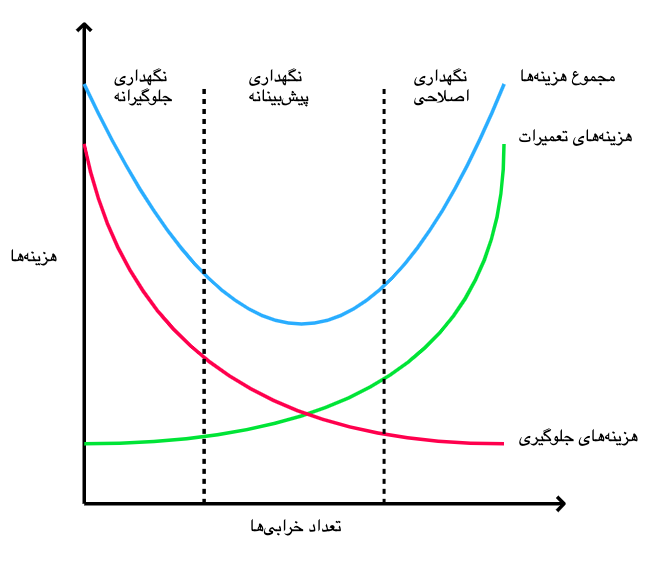
\includegraphics[width=.8\textwidth]{maintenance_comparison.png}}
\caption{مقایسه‌ی هزینه‌های انواع نگهد‌اری‌ها}
\label{fig:maintenance_comparison}
\end{figure}


\section{تعریف مسئله}
هدف از انجام این پروژه، پیاده‌سازی سیستمی برای اجراکردن نگهداری پیش‌بینانه بر روی گره‌های موجود در یک اینترنت اشیاء\LTRfootnote{Internet of Things} بهم پیوسته است. رویکردهای مختلفی برای این منظور تا کنون توسط محققان ابداع و مورد استفاده قرار گرفته شده است. از جمله‌ی این موارد می‌توان به تحلیل لرزش\LTRfootnote{Vibration Analysis} اشاره کرد. برای پیاده‌سازی این سیستم همانطور که در \cref{fig:workflow} به تصویر آمده ‌است، نیازمند آنیم که داده‌های لرزش مربوط به گره‌ها را که توسط یک سیستم قابل‌اتکا\LTRfootnote{Reliable} جمع‌آوری شده است، دریافت کرده و با جداکردن داده‌های پرت\LTRfootnote{Outlier Data}، از بین‌بردن تاثیر اختلال\LTRfootnote{Noise} ایجادشده توسط گرانش و خرابی یا درست‌ کارنکردن حسگر\LTRfootnote{Sensor} اندازه‌گیری لرزش، استخراج ویژگی‌\LTRfootnote{Feature Extraction}های مناسب برای انجام تحلیل روی داده و درنهایت پیشنهاد دادن مدلی برای نحوه‌ی یادگیری ماشین\LTRfootnote{Machine Learning} و تحلیل و مقایسه‌ی داده‌های بدست‌آمده با داده‌های برچسب‌دار\LTRfootnote{Labeled Data}، عمر باقی‌مانده\LTRfootnote{Remaining Useful Lifetime}‌ی دستگاه‌های مختلف را پیش‌بینی کنیم و بر اساس اعداد بدست‌آمده، اقدامات مناسب را برای انجام مراقبت‌های دوره‌ای انجام دهیم و از تحمیل‌شدن هزینه‌های جانبی در آینده جلوگیری کنیم\cite{jung2017vibration}. برای راحتی استفاده از سیستم طراحی‌شده، مستقرساختن\LTRfootnote{Deploy} سرویس توسعه‌یافته‌شده روی ابر\LTRfootnote{Cloud} و همچنین احراز هویّت مدیر\LTRfootnote{Admin}ان و دروازه\LTRfootnote{Gateway}‌های ارسال‌کننده داده‌ی لرزش کارگزار\LTRfootnote{Server}ی نیز پیاده خواهد شد.

\begin{figure}[!h]
\centerline{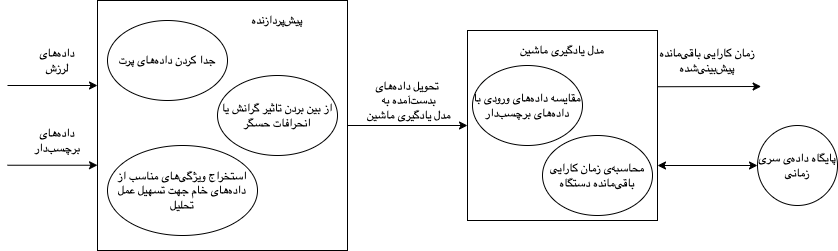
\includegraphics[width=1\textwidth]{workflow.png}}
\caption{نمودار جریان کار}
\label{fig:workflow}
\end{figure}


\section{کارهای مشابه}
نگهداری و تعمیرات پیش‌بینانه نسبتاً موضوع نو ظهوری است و عمر کمتری را نسبت به انواع دیگر نگهداری‌های موجود دارد. اما با این‌حال تا به امروز تلاش‌های قابل‌توجهی برای بکارگیری این نوع از نگهداری در سطح دنیا صورت گرفته است که در اینجا به مواردی که رویکردهای جالبی داشته‌اند اشاره خواهیم کرد. در \cite{tinga2010application} مدلی براي خرابی قطعات مبتنی بر ميزان استفاده از تجهيزات و بار داخلی آنها ارائه شده‌است اما مدل ارائه‌شده محدود به يک مدل تجهيزات است و براي استفاده در ساير مدل‌ها نظارت مجدد لازم است. در \cite{wu2007neural} روندی مبتنی بر شبكه‌های عصبی جهت پيش‌بينی عمر مفيد باقی‌مانده تجهيزات چرخشی ارائه شده‌است اما تنها مختص به اين دسته از تجهيزات است. در \cite{kaiser2009predictive} رويكردی مبتنی بر شبكه عصبی جهت پيش‌بينی زمان نگهداری و تعميرات تجهيزات بر اساس مدل خرابی و كارايی آنها ارائه می‌شود اما در یک محيط شبيه‌سازی‌شده و كنترل‌شده آزمايش شده‌است و در هنگام استفاده در محيط واقعی غيرعملی است.

 بطور كلی در پژوهش‌های يادشده روندهای در پیش‌گرفته‌شده برای پیش‌بینی خرابی و زمان آن، مختص نوع خاصی از تجهيزات است و در يک محيط آزمايشگاهی و كنترل‌شده ارزيابی شده‌اند. در حالی‌كه در اين پروژه با استفاده از داده‌های جمع‌آوری‌شده از قطعات مختلف سعی كرده‌ايم رويكردی كلی و مناسب محيط واقعی و صنعتی ارائه دهيم. همچنین شایان ذکر است که در هیچ‌کدام از پروژه‌های یاد‌شده، سیستم طراحی‌شده روی ابر مستقر نشده‌اند و سرویس‌هایی همانند احراز هویت و برنامه‌ی تحت وب برای آنها طراحی نشده است. این در حالی است که در این پروژه قصد بر این بوده که سیستمی کلی برای مدیریت بهتر قطعات با جلوه‌ای مناسب طراحی گردد و توسعه یابد.

\chapter{تکنولوژی‌های استفاده‌شده}

در این فصل تکنولوژی‌ها و چارچوب\LTRfootnote{Framework}‌های اصلی دخیل در توسعه این دستگاه را به طور دقیق مورد بررسی قرار می‌دهیم.

\section{‌‌زبان برنامه‌نویسی}
برای انتخاب زبان برنامه‌نویسی مناسب برای توسعه مدل یادگیری ماشین شرح‌داده شده، باید معیارهای متفاوتی را در نظر گرفت. برای این منظور زبان پایتون\LTRfootnote{\href{https://docs.python.org/3/}{Python}} را برگزیدیم. مواردی همچون داشتن چارچوب‌ها و کتابخانه‌های قدرتمند یادگیری ماشین، توسعه‌ی آسان و سریع و محبوبیت بالا از دلایل اصلی انتخاب پایتون به عنوان زبان اصلی برای توسعه‌ی سرویس یادگیری ماشین می‌باشد. همچنین شایان ذکر است که چون کارگزار اصلی جمع‌آوری اطلاعات لرزش به زبان پایتون نوشته شده است، استفاده از این زبان برای توسعه مدل یادگیری ماشین، باعث بهبود توسعه‌پذیری نیز می‌گردد. 

\subsection{زبان برنامه‌نویسی پایتون}
یک زبان برنامه‌نویسی عمومی و سطح بالا است که فلسفه طراحی آن بر روی خوانایی کد تأکید دارد. نحو\LTRfootnote{Syntax} پایتون به برنامه‌نویسان امکان می‌دهد تا مفاهیم را با تعداد کمتری خط کد نسبت به زبان‌هایی مانند سی\LTRfootnote{C Programming Language} بیان کنند و این زبان ساختارهایی را فراهم می‌کند که برنامه‌های واضح و قابل فهم را در هر دو مقیاس کوچک و بزرگ فراهم می‌سازد\cite{van2007python}. یکی از مشخصه‌های مهم پایتون این است که از چندین الگو\LTRfootnote{Paradigm}ی برنامه‌نویسی، از جمله شیءگرا\LTRfootnote{Object Oriented Programming (OOP)} و تابعی یا روش‌های رویه‌ای، پشتیبانی می‌کند. پایتون سیستم نوع پویا و مدیریت خودکار حافظه را پشتیبانی می‌کند و کتابخانه‌های استاندارد و جانبی بزرگ و جامع دارد. مفسرهای پایتون برای بسیاری از سیستم‌عامل‌ها در دسترس هستند\cite{srinath2017python}. از جمله مهم‌ترین ویژگی‌های پایتون می‌توان به موارد زیر اشاره کرد.

\begin{itemize}

\item \textbf{سادگی}: پایتون یک زبان برنامه‌نویسی بسیار سطح بالا است که منابع زیادی برای یادگیری آن وجود دارد. پایتون از ابزارهای شخص ثالث متنوعی پشتیبانی می‌کند که استفاده از آن را بسیار آسانتر می‌کند و کاربران را ترغیب می‌کند تا ادامه دهند\cite{srinath2017python, sharma2020python}.

\item \textbf{متن‌باز بودن\LTRfootnote{Open Source}}: اگرچه تمام حقوق این زبان برنامه‌نویسی متعلق به سازمان پایتون است، اما درحال‌ حاضر به عنوان یک نرم‌افزار متن‌باز وجود دارد و هیچ محدودیتی در استفاده، تغییر و توزیع آن وجود ندارد. می‌توان به آزادی از پایتون استفاده کرد و آن را برای استفاده شخصی و یا تجاری توزیع کرد. نه تنها می‌توان نرم‌افزاری که با آن نوشته شده است را استفاده و توزیع کرد، بلکه حتی می‌توان تغییراتی در خود کد منبع پایتون اعمال کرد. همچنین شایان ذکر است که پایتون یک جامعه بزرگ و پویا دارد که در هر نسخه آن را بهبود می‌بخشد\cite{srinath2017python, sharma2020python}.

\item \textbf{کتابخانه‌ها و چارچوب‌ها}: پایتون دارای یک سری کتابخانه‌های استاندارد و چارچوب‌های متنوع است که کار برنامه‌نویسان را بشدت راحت می‌کند، زیرا نیازی نیست تمام کدنویسی را خود برنامه‌نویس انجام دهد. کتابخانه‌های استاندارد در پایتون به خوبی تست شده‌اند و توسط هزاران نفر استفاده می‌شوند. بنابراین، می‌توان اطمینان داشت که استفاده از این کتابخانه‌ها توانایی ایجاد خرابی در برنامه‌های شما را ندارند\cite{srinath2017python, sharma2020python}.

\end{itemize}

حال به بررسی معایب پایتون می‌پردازیم. نکته‌ی قابل توجه در این قسمت این است که اگر معایب نام‌برده شده تاثیر زیادی در کیفیت خدمت ارائه‌شده به کاربر بگذارند، استفاده از پایتون اصلا توصیه نمی‌شود و باید به دنبال جایگزینی مناسب گشت. از جمله کاستی‌های پایتون عبارت‌اند از:

\begin{itemize}

\item \textbf{کندی}: به عنوان یک زبان با نوع پویا، پایتون به دلیل انعطاف‌پذیری بالا، کند عمل می‌کند، زیرا ماشین باید بسیاری از مراجعات را انجام دهد تا از تعریف چیزی مطمئن شود و این باعث کاهش عملکرد پایتون می‌شود\cite{srinath2017python, sharma2020python}.

\item \textbf{دشواری فرایند نگهداری\LTRfootnote{Maintaining}}: به دلیل اینکه پایتون یک زبان با نوع پویا است، یک چیز ممکن است به راحتی به معنای متفاوتی در تک‌نمایی متفاوت تفسیر شود. با افزایش اندازه و پیچیدگی یک برنامه پایتون، نگهداری آن ممکن است دشوار شود. با کمک تست‌های واحد\LTRfootnote{Unit Tests} می‌توان تا حدی این از وقوع این مشکل جلوگیری کرد\cite{srinath2017python, sharma2020python}.

\end{itemize}



\section{چارچوب‌ها و کتاب‌خانه‌ها}
در این پروژه از چارچوب فست‌ای‌پی‌آی\LTRfootnote{\href{https://fastapi.tiangolo.com/}{FastAPI}} برای دریافت درخواست‌ها و ارسال نتایج پیش‌بینی استفاده‌شده است(لوگوی مربوط به این چارچوب در \cref{fig:fastapi_logo}\cite{tiangoloFastAPI} آورده‌شده است). این سرویس به عنوان یک بسته\LTRfootnote{Package}ی پایتونی به کارگزار\LTRfootnote{Server} اصلی اضافه شده است. همچنین برای پیاده‌سازی مدل و انجام محاسبات ریاضی و ماتریسی از کتابخانه‌های نام‌پای\LTRfootnote{\href{https://numpy.org/}{NumPy}} و سایکیت\LTRfootnote{\href{https://scikit-learn.org/}{Scikit-Learn}} بهره برده شده است. در بخش‌های بعد به معرفی مختصر هر کدام از این موارد خواهیم پرداخت. لازم به ذکر است که جهت خوانایی بیشتر، از معادل انگلیسی این کتاب‌خانه‌ها برای اشاره به اسم آنها استفاده خواهیم کرد.

\subsection{چارچوب \lr{FastAPI}}
یک چارچوب مدرن با عملکرد عالی برای طراحی وب است که برای پایتون توسعه داده‌شده است. از ویژگی‌های کلیدی \lr{FastAPI} می‌توان به موارد زیر اشاره کرد\cite{tiangoloFastAPI}.

\begin{figure}[!h]
\centerline{
\includegraphics[width=\textwidth]{fastapi_logo.png}}
\caption{لوگوی \lr{FastAPI}\cite{tiangoloFastAPI}}
\label{fig:fastapi_logo}
\end{figure}
\begin{itemize}

\item \textbf{سریع‌بودن}: همانطور که در قسمت‌های قبل بدان اشاره شده، یکی از معایب پایتون کند بودن می‌باشد. نکته‌ی قابل توجه در اینجا این است که با وجود اینکه یکی از چارچوب‌های پایتون است، اما \lr{FastAPI} بسیار سریع است و کارایی و عملکرد بسیار بالایی را در اختیار می‌گذارد.

\item \textbf{سادگی توسعه}: بدلیل اینکه این زبان از نحو پایتون برای توسعه بهره می‌برد، سرعت توسعه‌دهنده برای ایجاد برنامه را دو تا سه برابر نسبت به چارچوب‌های دیگر برای توسعه برنامه‌ی تحت وب افزایش می‌دهد.

\item \textbf{کوتاه‌بودن}: این ویژگی باعث می‌شود که تکرار کد به حداقل میزان ممکن برسد و این خود منجر به این می‌شود که اشکالات\LTRfootnote{Bugs} کمتری که منشاء آن برنامه‌نویس هستند پیش بیایند.

\end{itemize}

\subsection{کتاب‌خانه‌ی \lr{NumPy}}
\lr{NumPy} یکی از معروف‌ترین کتاب‌خانه‌های زبان پایتون برای پردازش علمی و عددی است و اکنون، ۱۸ سال پس از عرضه، همانطور که در \cref{fig:numpy_related_packs}\cite{van2011numpy} مشخص است، مبنای بسیاری از کتاب‌خانه‌های دیگر پایتون است. این کتاب‌خانه‌ی متن‌باز توسط جامعه‌ی پایتونی توسعه‌یافته است و یک شیء آرایه چندبعدی پایتون به همراه تابع‌هایی که روی آن عمل می‌کنند، ارائه می‌دهد. \lr{NumPy} بدلیل سادگی ذاتی، به عنوان ساختار اصلی مبادله اطلاعات آرایه‌ای در پایتون مورد استفاده قرار می‌گیرد\cite{harris2020array}. آرایه‌ی نام‌پای در واقع یک ساختمان داده است که به صورت بهینه آرایه‌های چند‌بعدی پایتون را ذخیره می‌کند و به آن‌ها دسترسی پیدا می‌کند. همچنین توانایی انجام محاسبات علمی مختلف را بر روی این آرایه‌ها برای ما فراهم می‌کند. این ساختمان داده شامل یک اشاره‌گر\LTRfootnote{Pointer} به حافظه و تعدادی فراداده\LTRfootnote{Metadata} برای تفسیر داده‌های موجود در آرایه است\cite{harris2020array, van2011numpy}.

\begin{figure}[!h]
\centerline{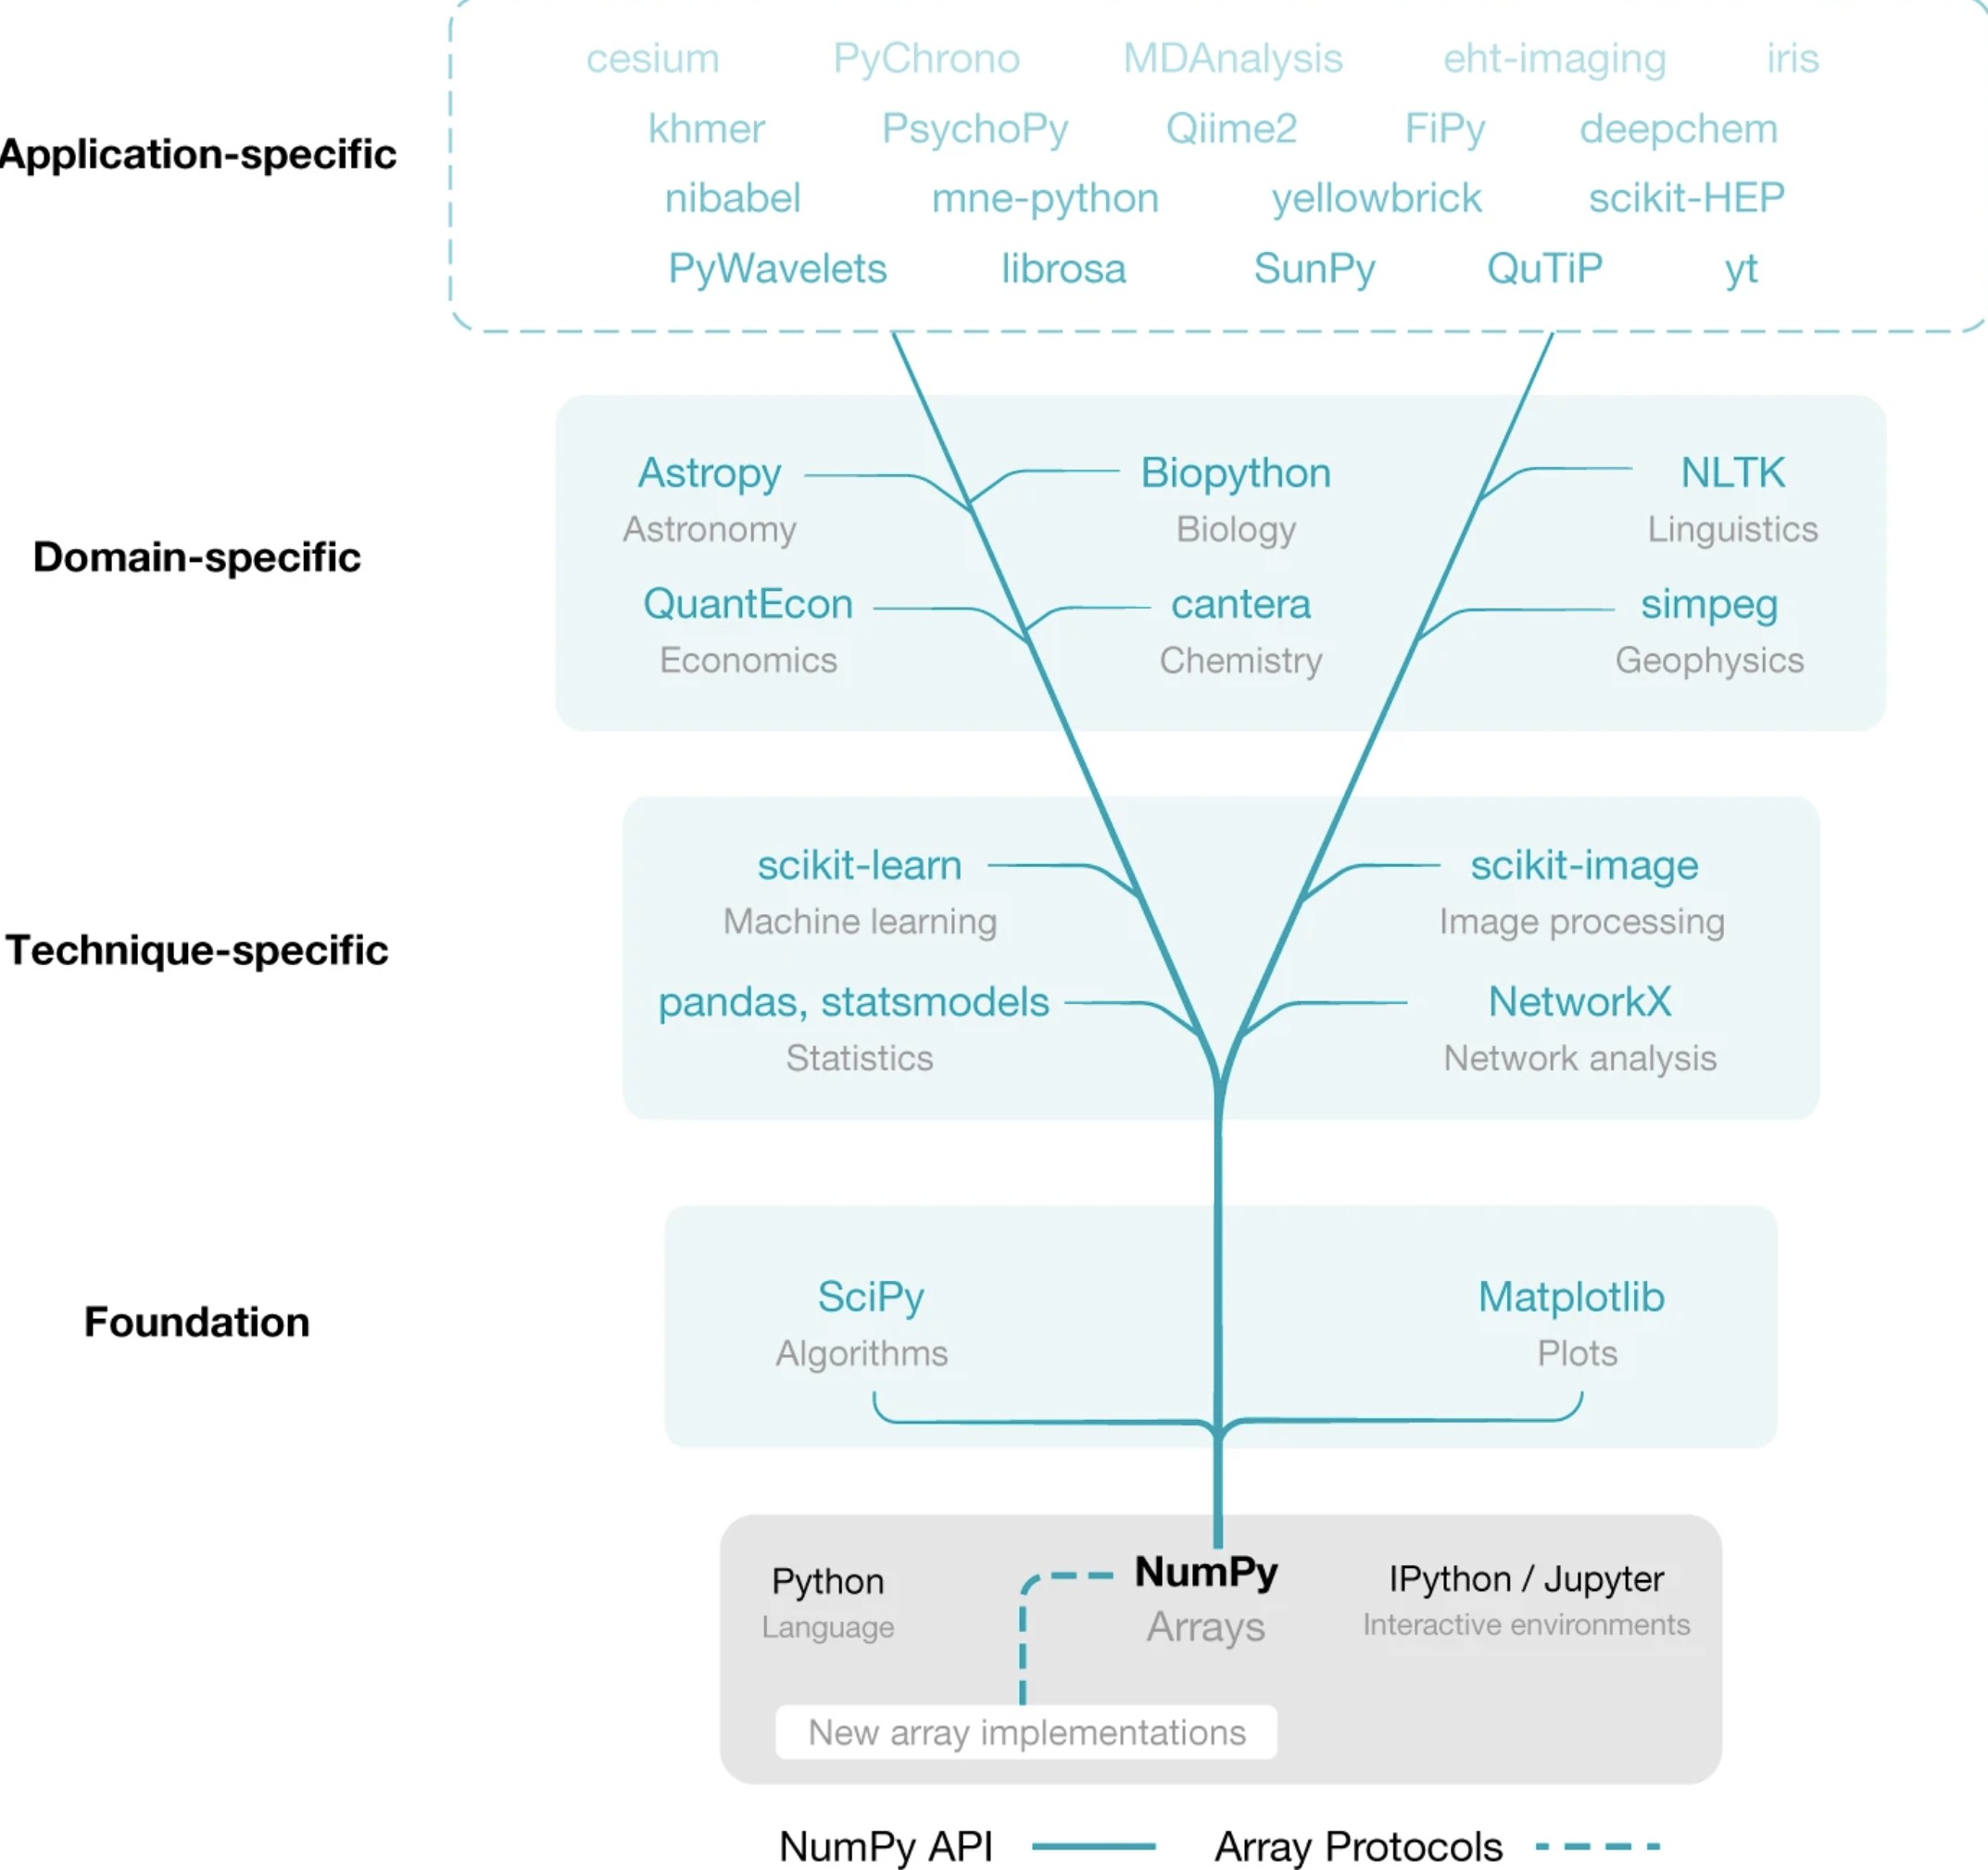
\includegraphics[width=\textwidth]{numpy_related_packs.png}}
\caption{گراف وابستگی کتاب‌خانه‌های پایتون به \lr{NumPy}\cite{van2011numpy}}
\label{fig:numpy_related_packs}
\end{figure}

\subsection{کتاب‌خانه‌ی \lr{Scikit-Learn}} 
\lr{Scikit-Learn}، جامع‌ترین و بزرگ‌ترین بسته یادگیری ماشین منبع‌باز در پایتون است. چون یادگیری ماشین اغلب به عنوان یک جزء از یک برنامه عمومی‌تر (همانند پروژه‌ی کنونی که به عنوان یک سرویس در وب توسعه داده‌شده است) استفاده می‌شود، ایده‌آل است که از همان زبان برنامه‌نویسی استفاده شود تا به‌صورت یکپارچه با سایر بخش‌های برنامه هماهنگ شود. با استفاده از قابلیت‌های گسترده پایتون، \lr{Scikit-Learn} به عنوان یک بسته محبوب برای برنامه‌های مرتبط با یادگیری ماشین در حال رشد است\cite{hao2019machine}. این کتاب‌خانه شامل توابع و اشیاء فراوانی برای مسائل طبقه‌بندی، رگرسیون، تقریب ماتریس کوواریانس، کاهش بعد و پیش‌پردازش داده‌ی خام می‌باشد\cite{kramer2016scikit}. اگرچه پایتون یک زبان برنامه‌نویسی تفسیری است، اما بیشتر روش‌های یادگیری ماشین در \lr{Scikit-Learn} بر پایه کتابخانه‌های دودویی کامپایل شده است که در ابتدا با زبان‌های فورتران\LTRfootnote{Fortran}، سی یا سی‌پلاس‌پلاس\LTRfootnote{C++} برنامه‌نویسی شده‌اند. این پیاده‌سازی‌های مبتنی بر دودویی‌ها به طور قابل توجهی کارایی محاسبات را بهبود می‌بخشند\cite{hao2019machine, kramer2016scikit}.

\section{جمع‌بندی و نتیجه‌گیری}
در این بخش، به تکنولوژی‌ها و چارچوب‌های اصلی استفاده‌شده برای توسعه‌ی مدل یادگیری ماشین اشاره کردیم. همانطور که در طول فصل بدان اشاره شد، زبان پایتون بدلیل دارا بودن غنی‌ترین کتابخانه‌های مربوط به محاسبات و یادگیری ماشین منطقی‌ترین انتخاب ممکن برای برگزیدن زبان توسعه‌ی مدل و سرویس هوش‌مصنوعی بود. دارا بودن چارچوب‌های با کارایی بالا برای توسعه برنامه‌ی وب نیز دیگر دلیل مهم برای انتخاب پایتون است.  
\chapter{استقرار مدل یادگیری ماشین}

پس از پیاده‌سازی مدل یادگیری ماشین، نیاز است که به طریقی سیستم را در دسترس همگان قرار داد تا بتوان از مزایای آن استفاده کرد. شرکت‌های ارائه‌دهنده‌ی خدمات ابری\LTRfootnote{Cloud Services Providers} یا به اختصار \lr{CPS}، گزینه‌ی مناسبی برای این نیاز می‌باشد. برای این منظور، ما این پروژه را پس از پیاده‌سازی، توسط سرویس زیرساخت به عنوان خدمت\LTRfootnote{Infrastructure as a Service (IaaS)} مستقر کردیم.


\section{زیرساخت به عنوان خدمت}
در این مدل، سرویس‌دهنده ابر یا \lr{CPS} مجموعه‌ای از منابع محاسباتی مجازی شده را در ابر فراهم می‌کند (مانند پهنای باند شبکه، ظرفیت ذخیره‌سازی، حافظه، قدرت پردازش). مسئولیت مشتری در این حالت این است که سیستم‌عامل و برنامه‌های نرم‌افزاری را روی این منابع مجازی اجرا و نگهداری کند. زیرساخت به عنوان خدمت یا \lr{IaaS} از فناوری مجازی‌سازی استفاده می‌کند تا منابع فیزیکی را به منابع منطقی تبدیل کند که مشتریان می‌توانند به صورت پویا از آنها استفاده کنند و آنها را هنگام نیاز ایجاد و آزاد کنند\cite{youssef2012exploring}. در \cref{fig:different_cloud_services} نمای کلی سرویس‌های مختلف موجود در یک سیستم ابری را مشاهده می‌کنیم. همانطور که مشخص است در \lr{IaaS}، کاربر بیشترین کنترل را بر روی منابع در اختیار گذاشته‌شده دارد\cite{serrano2015infrastructure}.



\begin{figure}[!h]
\centerline{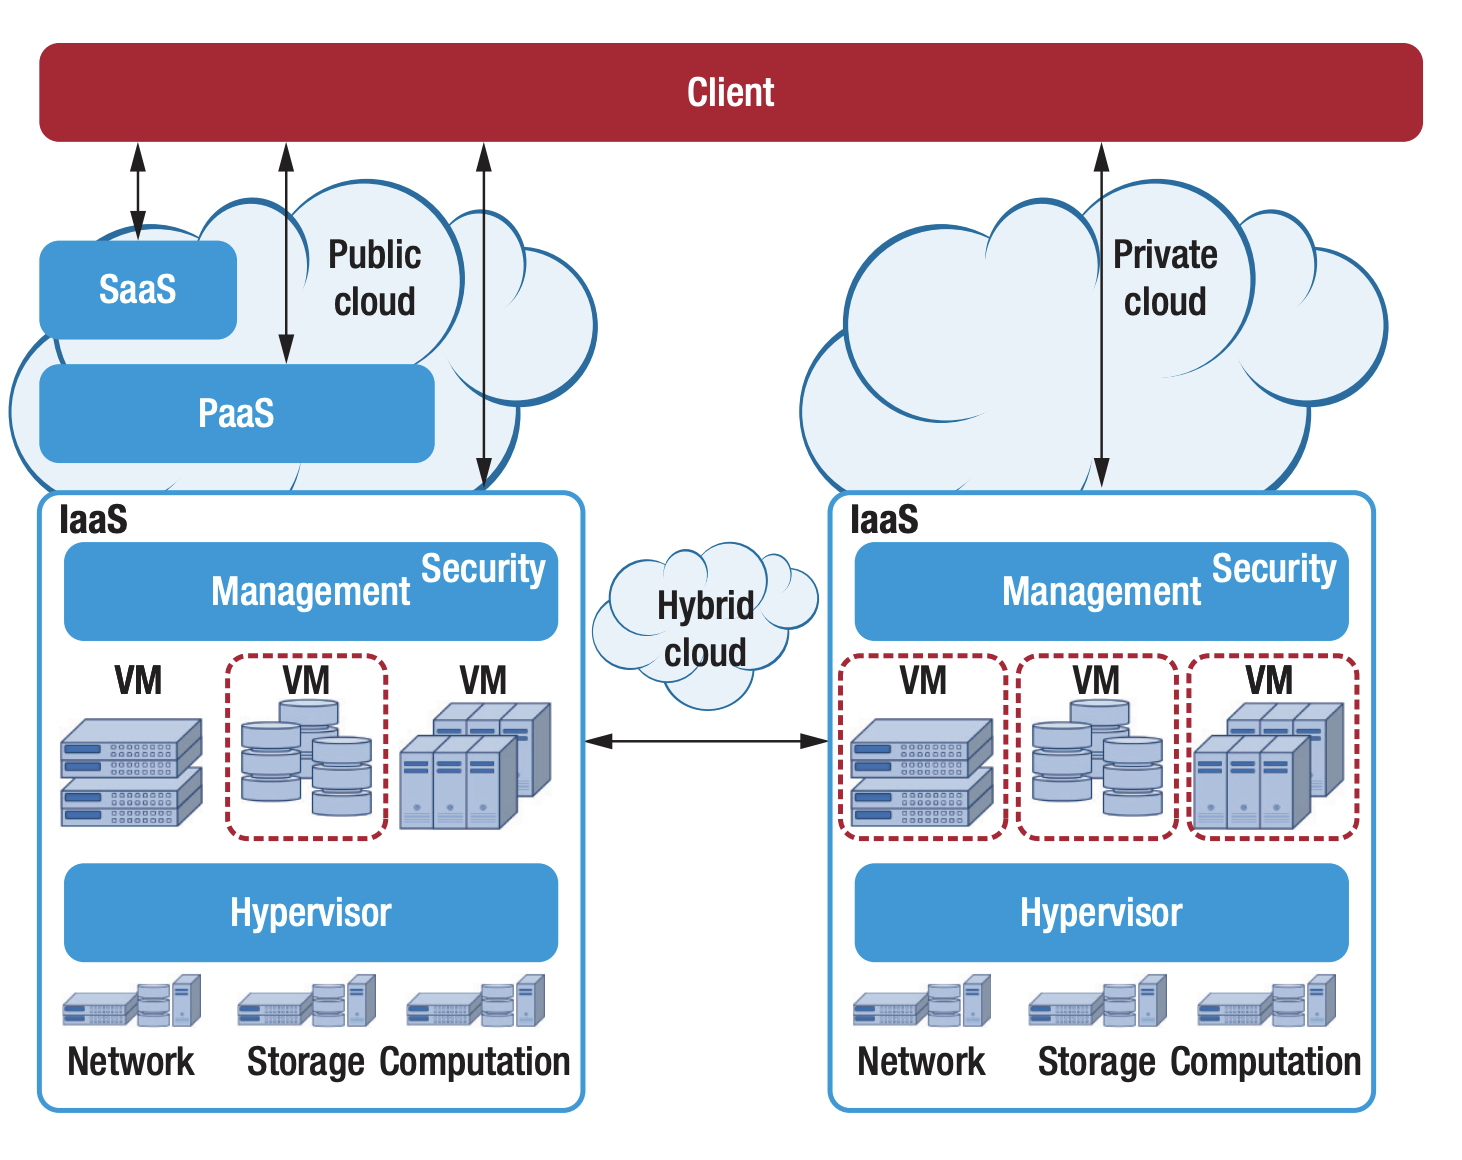
\includegraphics[width=\textwidth]{different_cloud_services.png}}
\caption{انواع سرویس‌های ارائه‌شده توسط شرکت‌های خدمات ابری}
\label{fig:different_cloud_services}
\end{figure}


\section{انواع روش‌های استقرار}
 روش‌های مختلفی برای استقرار و استفاده از مدل‌های یادگیری هوش مصنوعی مورد استفاده قرار می‌گیرند که از بین اینها چهار روش نشان داده‌ شده در \cref{fig:ml_model_deployments} مرسوم‌تر هستند\cite{kaggleMLdeployments}:

\begin{figure}[!h]
\centerline{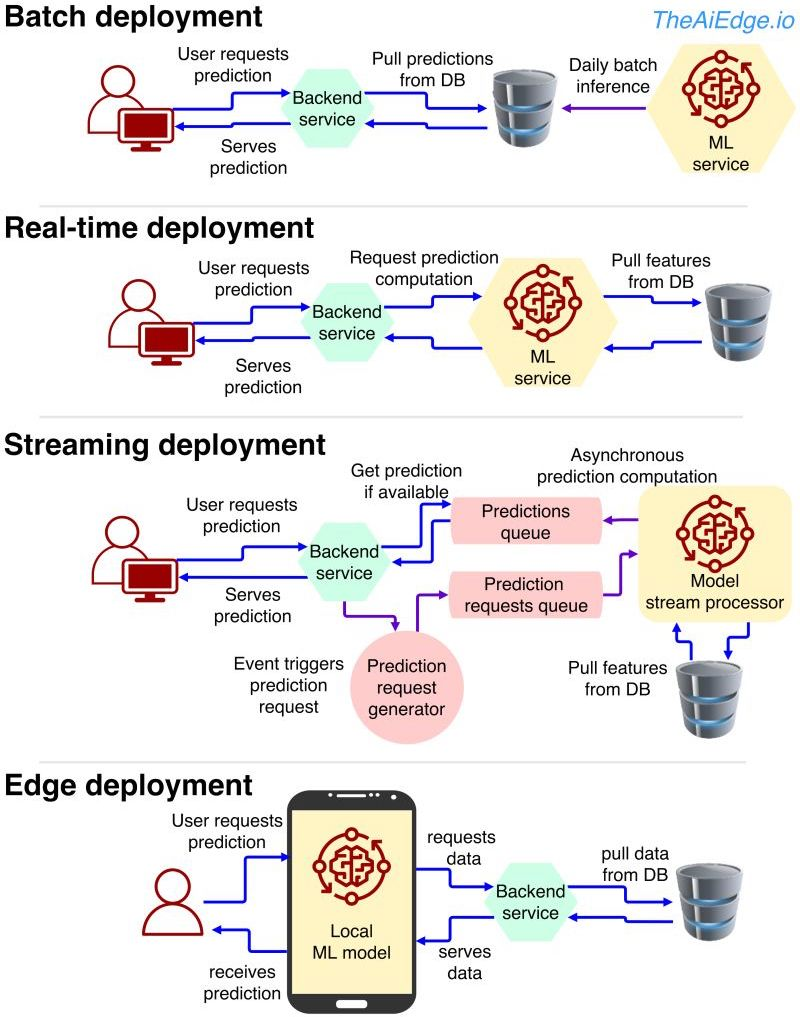
\includegraphics[width=.5\textwidth]{ml_model_deployments.png}}
\caption{انواع روش‌های استقرار مدل‌های یادگیری ماشین}
\label{fig:ml_model_deployments}
\end{figure}

\begin{itemize}

\item \textbf{پیاده‌سازی دسته‌ای\LTRfootnote{Batch Deployment}}: پیش‌بینی‌ها به فاصله‌های زمانی مشخص محاسبه می‌شوند و پیش‌بینی‌های حاصل در پایگاه داده ذخیره می‌شوند و به راحتی می‌توان آنها را در صورت نیاز بازیابی کرد. با این حال، نمی‌توان از داده‌های بروزتر استفاده کرد و پیش‌بینی‌ها می‌توانند به سرعت منسوخ شوند\cite{singh2021deploy, pacheco2018towards}.

\item \textbf{پیاده‌سازی بی‌درنگ\LTRfootnote{Real-Time Deployment}}: در این نوع از استقرار، درخواست کاربر برای گرفتن جدید‌ترین پیش‌بینی‌ها به عنوان یک راه‌انداز\LTRfootnote{Trigger} توسط رابط برنامه‌نویسی\LTRfootnote{Application Programming Interface (API)} اچ‌تی‌تی‌پی\LTRfootnote{Hypertext Transfer Protocol (HTTP)} به کارگزار ارسال می‌شود. سپس سرویس یادگیری ماشین که به عنوان افزونه‌ای در سمت کارگزار توسعه یافته است، شروع به کار می‌کند و جدیدترین نتایج پیش‌بینی را تولید و ذخیره می‌کند و به سمت کاربر به عنوان نتیجه ارسال می‌کند. مشکل اصلی این روش قرارگیری مدل یادگیری ماشین، کند بودن روند یادگیری و پیش‌بینی است که منجر به منتظر ماندن کاربر می‌گردد. می‌توان با بهره‌گیری از فرآیند\LTRfootnote{Process}‌های چندریسمانی\LTRfootnote{Multi-Threaded} برای دریافت درخواست‌های کاربر و انجام مرحله‌ی یادگیری و پیش‌بینی مدل، تا حد زیادی این مشکل را برطرف کرد\cite{singh2021deploy, pacheco2018towards}.

\item \textbf{پیاده‌سازی جریانی\LTRfootnote{Streaming Deployment}}: این امکان را می‌دهد تا فرآیند ناهمزمان‌\LTRfootnote{Asynchronous}تری ایجاد شود. یک رویداد می‌تواند شروع فرآیند استنتاج را فراهم کند. این فرآیند در صف یک واسط پیام\LTRfootnote{Message Broker} مانند کافکا\LTRfootnote{Apache Kafka} قرار داده می‌شود و مدل یادگیری ماشینی در هنگام آماده شدن برای انجام درخواست، آن را انجام می‌دهد. این کار به سرویس پشتیبانی فرصت می‌دهد و با فرآیند صف بهینه، قدرت محاسباتی بسیاری را صرفه‌جویی می‌کند. پیش‌بینی‌های حاصل شده نیز در صف قرار گرفته و در صورت نیاز توسط سرویس‌های پشتیبانی مصرف می‌شوند. از مزیت‌های این روش نسبت به روش بی‌درنگ، می‌توان به کم‌شدن تاخیر پاسخ‌دهی به کاربران اشاره کرد\cite{singh2021deploy, pacheco2018towards}.

\item \textbf{پیاده‌سازی لبه‌ای\LTRfootnote{Edge Deployment}}: در این روش استقرار، مدل مستقیماً بر روی کلاینت نصب می‌شود، مانند مرورگر وب، یک تلفن همراه یا محصولات اینترنت اشیاء. این کار باعث رسیدن به سریع‌ترین استنتاج می‌شود، اما معمولاً مدل‌ها باید به اندازه کافی کوچک باشند تا بتوانند در سخت‌افزارهای کوچکتر نصب شوند\cite{kaggleMLdeployments}.

\end{itemize}

بدلیل اینکه گره‌های موجود در شبکه‌ی اشیاء دارای توان پردازشی محدود هستند و اینکه ماهیت مدل هوش‌ مصنوعی مربوط به حوزه‌ی کاری پیش‌بینی عمر دستگاه‌ها بدین‌گونه است که حتما باید از داده‌های مربوط به همه‌ی گره‌های موجود استفاده کرد، با توجه به گزینه‌های مطرح‌شده برای استقرار مدل هوش مصنوعی توسعه‌داده شده و همچنین مزایا و معایب هر کدام، از روش استقرار بی‌درنگ برای ارائه و بکارگیری مدل هوش مصنوعی در این پروژه استفاده شده است. به طور دقیقتر، مدل هوش مصنوعی به عنوان یک سرویس اضافی برای کارگزار اصلی توسعه‌ داده‌شده در پروژه‌ی مرتبط 
به این پروژه تعبیه شده است. 
\chapter{پیاده‌سازی و توسعه مدل یادگیری ماشین}

در این فصل روش پیاده‌سازی مدل هوش مصنوعی را به تفصیل شرح خواهیم داد. ابتدا فرضیات و داده‌های ورودی و آماده‌ی تحلیل را مشخص کرده و نماد هر کدام را که تا انتهای این نوشته از آنها استفاده خواهیم کرد، مشخص می‌کنیم. در قسمت بعد مراحل پیش‌پردازش\LTRfootnote{Preprocess} را که روی این داده‌ها انجام می‌شود به ترتیب توضیح می‌دهیم و سپس ویژگی‌هایی که نیاز داریم از این داده‌های خام دربیاوریم را توضیح می‌دهیم و نحوه‌ی استخراج این ویژگی‌ها را نمایان می‌کنیم. در مرحله‌ی نهایی روش آموزاندن و یادگیری مدل هوش مصنوعی را بر اساس این ویژگی‌ها شرح می‌دهیم.


\section{توضیح مسئله}
با توجه به اینکه سیستم یادگیری ماشین بر اساس اطلاعات حسگرهای لرزش عمل می‌کند، برای داشتن کمترین خطا در عملیات پیش‌بینی باید فرضیاتی را پیش از طراحی و پیاده‌سازی سیستم در نظر داشته باشیم. اولاً نمونه‌های بدست‌آمده برای حسگرهای متفاوت بازه‌های زمانی مختلف را در بر می‌گیرند و همگن نیستند. ثانیاً این داده‌های دارای انحرافاتی در اندازه‌گیری بدلیل وجود گرانش یا خرابی حسگر هستند. ثالثاً وضعیت ابتدایی هر یک از گره‌هایی که می‌خواهیم اطلاعات لرزش آنها را جمع‌آوری و تحلیل کنیم یکی نیستند\cite{jung2017vibration}. با توجه به نکاتی که مطرح کردیم، پیاده‌کردن یک سیستم پیش‌پردازش و استخراج‌کننده‌ی ویژگی‌های مناسب، الزامی است. در \cref{table:notation_description} توضیحات نشانه‌گذاری داده‌ی مربوط به این مسئله را می‌بینیم.

\begin{table}[h!]
  \begin{center}
    \caption{توضیحات نشانه‌گذاری داده‌ها}
    \label{table:notation_description}
    \begin{tabular}{|c|c|} % <-- Alignments: 1st column left and 2nd right with vertical lines in between
    	\hline
تعداد کل گره‌ها & $N$\\
    	\hline
 تعداد کل اندازه‌گیری‌ها & $M$\\
    	\hline
   تعداد کل نمونه‌های یک اندازه‌گیری & $K$\\
    	\hline
گره $n$ ام & $n$\\
 	\hline
اندازه‌گیری $m$ ام & $m$\\
 	\hline
نمونه‌ی $k$ ام یک اندازه‌گیری & $k$\\
 	\hline
بردار سه‌بعدی مربوط به اندازه‌گیری لرزش & $a_{nmk}$\\
 	\hline
بردار $k$بعدی مربوط به لرزش در محور $l \in \{x, y, z\}$  & $a^l_{nm}$\\
 	\hline
    \end{tabular}
  \end{center}
\end{table} 

\section{پیش‌پردازش}
این بخش وظیفه دارد قبل از انجام تحلیل داده، انحرافات و داده‌های پرت\LTRfootnote{Outlier Data} را از داده‌ی خام جدا کرده و داده‌ی قابل پردازش را به لایه‌ی بعد که لایه‌ی استخراج ویژگی‌ است تحویل دهد.

\subsection{از بین بردن انحرافات}
 حسگرهای کم‌هزینه \lr{MEMS} ،که داده‌های جمع‌آوری‌شده برای این پروژه توسط این نوع از حسگرها تأمین شده است، غالباً با گذشت زمان دچار انحرافاتی در اندازه‌گیری خواهند شد که منجر به اضافه یا کم شدن یک مقدار شتاب غیر صفر در اندازه‌گیری‌هایشان خواهد شد. از طرفی وجود گرانش، تاثیراتی روی اندازه‌گیری‌ها خواهد داشت و موجب ایجاد انحرافاتی رو به بالا یا پایین در این مقادیر خواهد شد\cite{jung2017vibration}. برای از بین بردن این مشکل همانطور که در \cref{eq:normalize} آورده شده است، از عادی‌کردن\LTRfootnote{Normalizing} داده با کم‌کردن میانگین مقادیر شتاب اندازه‌گیری شده در هر کدام از سه محور از مقادیر اندازه‌گیری‌شده استفاده کرد. لازم به ذکر است همانطور که مشخص است، $\hat{a}^l_{nm}$ نماد ماتریس عادی‌شده است.
\begin{equation}
\label{eq:normalize}
	\hat{a}^l_{nm}=a^l_{nm}-\sum_{k=1}^K \dfrac{a^l_{nmk}}{K}
\end{equation}


\subsection{از بین بردن داده‌های پرت}


\section{استخراج ویژگی‌ها}


\section{نحوه‌ی یادگیری مدل}
\chapter{پیاده‌سازی و توسعه مدل یادگیری ماشین}

در این فصل روش پیاده‌سازی مدل هوش مصنوعی را به تفصیل شرح خواهیم داد. ابتدا فرضیات و داده‌های ورودی و آماده‌ی تحلیل را مشخص کرده و نماد هر کدام را که تا انتهای این نوشته از آنها استفاده خواهیم کرد، مشخص می‌کنیم. در قسمت بعد مراحل پیش‌پردازش\LTRfootnote{Preprocess} را که روی این داده‌ها انجام می‌شود به ترتیب توضیح می‌دهیم و سپس ویژگی‌هایی که نیاز داریم از این داده‌های خام دربیاوریم را توضیح می‌دهیم و نحوه‌ی استخراج این ویژگی‌ها را نمایان می‌کنیم. در مرحله‌ی نهایی نحوه‌ی یادگیری مدل هوش مصنوعی و پیش‌بینی عمر باقی‌مانده‌ی دستگاه‌ها را بر اساس این ویژگی‌ها شرح می‌دهیم. در \cref{fig:analytics_structure}، قالب بسته‌ی هوش مصنوعی توسعه داده‌شده برای کارگزار اصلی را مشاهده می‌کنید که در این فصل به توضیح بخش‌های مختلف آن می‌پردازیم.

\begin{figure}[!h]
\centerline{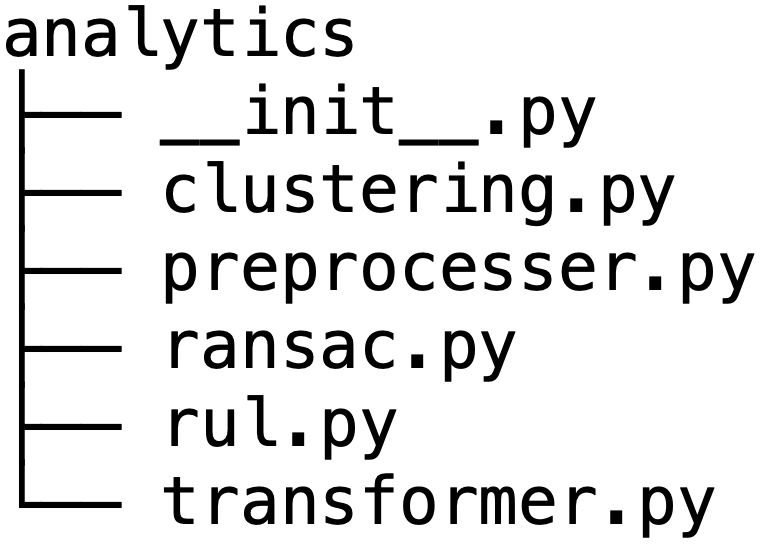
\includegraphics[width=0.4\textwidth]{analytics_structure.png}}
\caption{ساختار کلی بسته‌ی هوش مصنوعی}
\label{fig:analytics_structure}
\end{figure}


\section{توضیح مسئله}
با توجه به اینکه سیستم یادگیری ماشین بر اساس اطلاعات حسگرهای لرزش عمل می‌کند، برای داشتن کمترین خطا در عملیات پیش‌بینی باید فرضیاتی را پیش از طراحی و پیاده‌سازی سیستم در نظر داشته باشیم. اولاً نمونه‌های بدست‌آمده برای حسگرهای متفاوت بازه‌های زمانی مختلف را در بر می‌گیرند و همگن نیستند. ثانیاً این داده‌های دارای انحرافاتی در اندازه‌گیری بدلیل وجود گرانش یا خرابی حسگر هستند. ثالثاً وضعیت ابتدایی هر یک از گره‌هایی که می‌خواهیم اطلاعات لرزش آنها را جمع‌آوری و تحلیل کنیم یکی نیستند\cite{jung2017vibration}. با توجه به نکاتی که مطرح کردیم، پیاده‌کردن یک سیستم پیش‌پردازش و استخراج‌کننده‌ی ویژگی‌های مناسب، الزامی است. 

\begin{table}[h!]
  \begin{center}
    \caption{توضیحات نشانه‌گذاری داده‌ها}
    \label{table:notation_description}
    \begin{tabular}{|c|c|} % <-- Alignments: 1st column left and 2nd right with vertical lines in between
    	\hline
\textbf{توضیحات} & \textbf{نشانه}\\
    	\hline \hline
تعداد کل گره‌ها & $N$\\
    	\hline
 تعداد کل اندازه‌گیری‌ها & $M$\\
    	\hline
   تعداد کل نمونه‌های یک اندازه‌گیری & $K$\\
    	\hline
گره $n$ ام & $n$\\
 	\hline
اندازه‌گیری $m$ ام & $m$\\
 	\hline
نمونه‌ی $k$ ام یک اندازه‌گیری & $k$\\
 	\hline
بردار سه‌بعدی مربوط به اندازه‌گیری لرزش & $a_{nmk}$\\
 	\hline
بردار $k$بعدی مربوط به لرزش در محور $l \in \{x, y, z\}$  & $a^l_{nm}$\\
 	\hline
    \end{tabular}
  \end{center}
\end{table} 

\begin{table}[h!]
  \begin{center}
    \caption{برچسب‌های استفاده‌شده برای تعیین وضعیت دستگاه‌ها}
    \label{table:node_state_labels}
    \begin{tabular}{|c|c|} % <-- Alignments: 1st column left and 2nd right with vertical lines in between
    	\hline
\textbf{توضیحات} & \textbf{برچسب}\\
    	\hline \hline
دستگاه‌های نو که تازه تولید شده‌اند و آماده استفاده‌اند & $A$\\
    	\hline
دستگاه‌هایی که نو نیستند ولی هنوز مشغول کارکردن هستند & $B, C$\\
    	\hline
  دستگاه‌هایی خراب‌ شده‌اند یا در حال خرابی‌اند & $D$\\
    	\hline
    \end{tabular}
  \end{center}
\end{table}

در \cref{table:notation_description} توضیحات نشانه‌گذاری داده‌ی مربوط به این مسئله را می‌بینیم. همچنین در جهت مشخص کردن محدوده‌ی کاری این مسئله، از سه برچسب که در \cref{table:node_state_labels} مشخص شده‌اند، برای تعیین کردن وضعیت گره‌های موجود استفاده می‌کنیم.

\section{پیش‌پردازش}
این بخش وظیفه دارد قبل از انجام تحلیل داده، در ابتدا انحرافات و داده‌های پرت\LTRfootnote{Outlier Data} را از داده‌ی خام جدا کرده و داده‌ی قابل پردازش را به لایه‌ی بعد که لایه‌ی استخراج ویژگی‌ است تحویل دهد. در نهایت خروجی بخش پیش‌پردازنده، ویژگی‌هایی هستند که دستگاه یادگیری ماشین با تحلیل و بررسی آنها عملیات یادگیری و پیش‌بینی را انجام خواهد داد.

\subsection{از بین بردن انحرافات}
 حسگرهای کم‌هزینه \lr{MEMS} ،که داده‌های جمع‌آوری‌شده برای این پروژه توسط این نوع از حسگرها تأمین شده است، غالباً با گذشت زمان دچار انحرافاتی در اندازه‌گیری خواهند شد که منجر به اضافه یا کم شدن یک مقدار شتاب غیر صفر در اندازه‌گیری‌هایشان خواهد شد. از طرفی وجود گرانش، تاثیراتی روی اندازه‌گیری‌ها خواهد داشت و موجب ایجاد انحرافاتی رو به بالا یا پایین در این مقادیر خواهد شد\cite{jung2017vibration}. برای از بین بردن این مشکل همانطور که در \cref{eq:normalize} آورده شده است\cite{garcia2015data}، از هنجار‌کردن\LTRfootnote{Normalizing} داده با کم‌کردن میانگین مقادیر شتاب اندازه‌گیری شده در هر کدام از سه محور از مقادیر اندازه‌گیری‌شده استفاده کرده‌ایم. لازم به ذکر است همانطور که مشخص است، $\hat{a}^l_{nm}$ نماد ماتریس هنجار‌شده است.
\begin{equation}
\label{eq:normalize}
	\hat{a}^l_{nm}=a^l_{nm}-\sum_{k=1}^K \dfrac{a^l_{nmk}}{K}
\end{equation}


\subsection{از بین بردن داده‌های پرت}
در سیستم طراحی‌شده برای جمع‌آوری اطلاعات، ممکن است که تعدادی از حسگرها دچار مشکل شده باشند و داده‌ای که تحویل دروازه می‌دهند دقیق و در راستای داده‌های از قبل جمع‌آوری شده نباشد. به طور کلی، پایدار بودن میانگین شتاب دریافت‌شده از هر اندازه‌گیری، معیار خوبی برای تشخیص صحت و درستی اطلاعات جمع‌‌آوری شده است\cite{jung2017vibration}. به عبارتی دیگر، میانگین لرزش‌های اندازه گرفته‌شده نباید به طور ناگهانی بالا یا پایین روند و باید در همان حدود اندازه‌گیری‌های قبل باشند. برای جدا کردن این داده‌ها که اصطلاحا به آنها داده‌های پرت می‌گوییم، پیش از شروع یادگیری مدل، ابتدا میانگین شتاب جمع‌‌آوری ‌شده برای هر اندازه‌گیری موجود را در هر سه بعد حساب کرده و سپس با کمک یک الگوریتم خوشه‌بندی\LTRfootnote{Clustering}، این داده‌ها را جدا می‌کنیم.

برای انجام عملیات تشخیص داده‌های پرت، از الگوریتم خوشه‌بندی میانگین تغییر\LTRfootnote{Mean Shift} استفاده کرده‌ایم که الگوریتمی بر اساس تخمین تراکم هسته\LTRfootnote{Kernel Density Estimate} می‌باشد. در \cref{fig:density_based_clustering}\cite{carreira2015review} نمونه‌ای از یک الگوریتم خوشه‌بندی تراکم‌محور آورده شده است. روند کار این الگوریتم بدین صورت است که به ازای ورودی به صورت نقاط و پارامتر ورودی پهنای باند\LTRfootnote{Bandwidth}، الگوریتم به طور مکرر هر نقطه داده را به نزدیکترین مرکز خوشه اختصاص می‌دهد و جهت نزدیکترین مرکز خوشه بر اساس جایی که اکثر نقاط نزدیک در آن قرار دارند تعیین می‌شود. در هر بار تکرار، هر نقطه داده به جایی که بیشترین نقاط در آن قرار دارد، نزدیکتر می‌شود، که در نهایت به مرکز خوشه منجر خواهد شد. هنگامی که الگوریتم متوقف می‌شود، هر نقطه به یک خوشه اختصاص داده می‌شود. همانطور که گفته‌شد، این الگوریتم بغیر از پهنای باند به پارامتر دیگری نیاز ندارد. این امر سبب می‌شود که مواردی همانند تعداد و مراکز هر خوشه، توسط خود الگوریتم مشخص شوند\cite{carreira2015review}.

\begin{figure}[!h]
\centerline{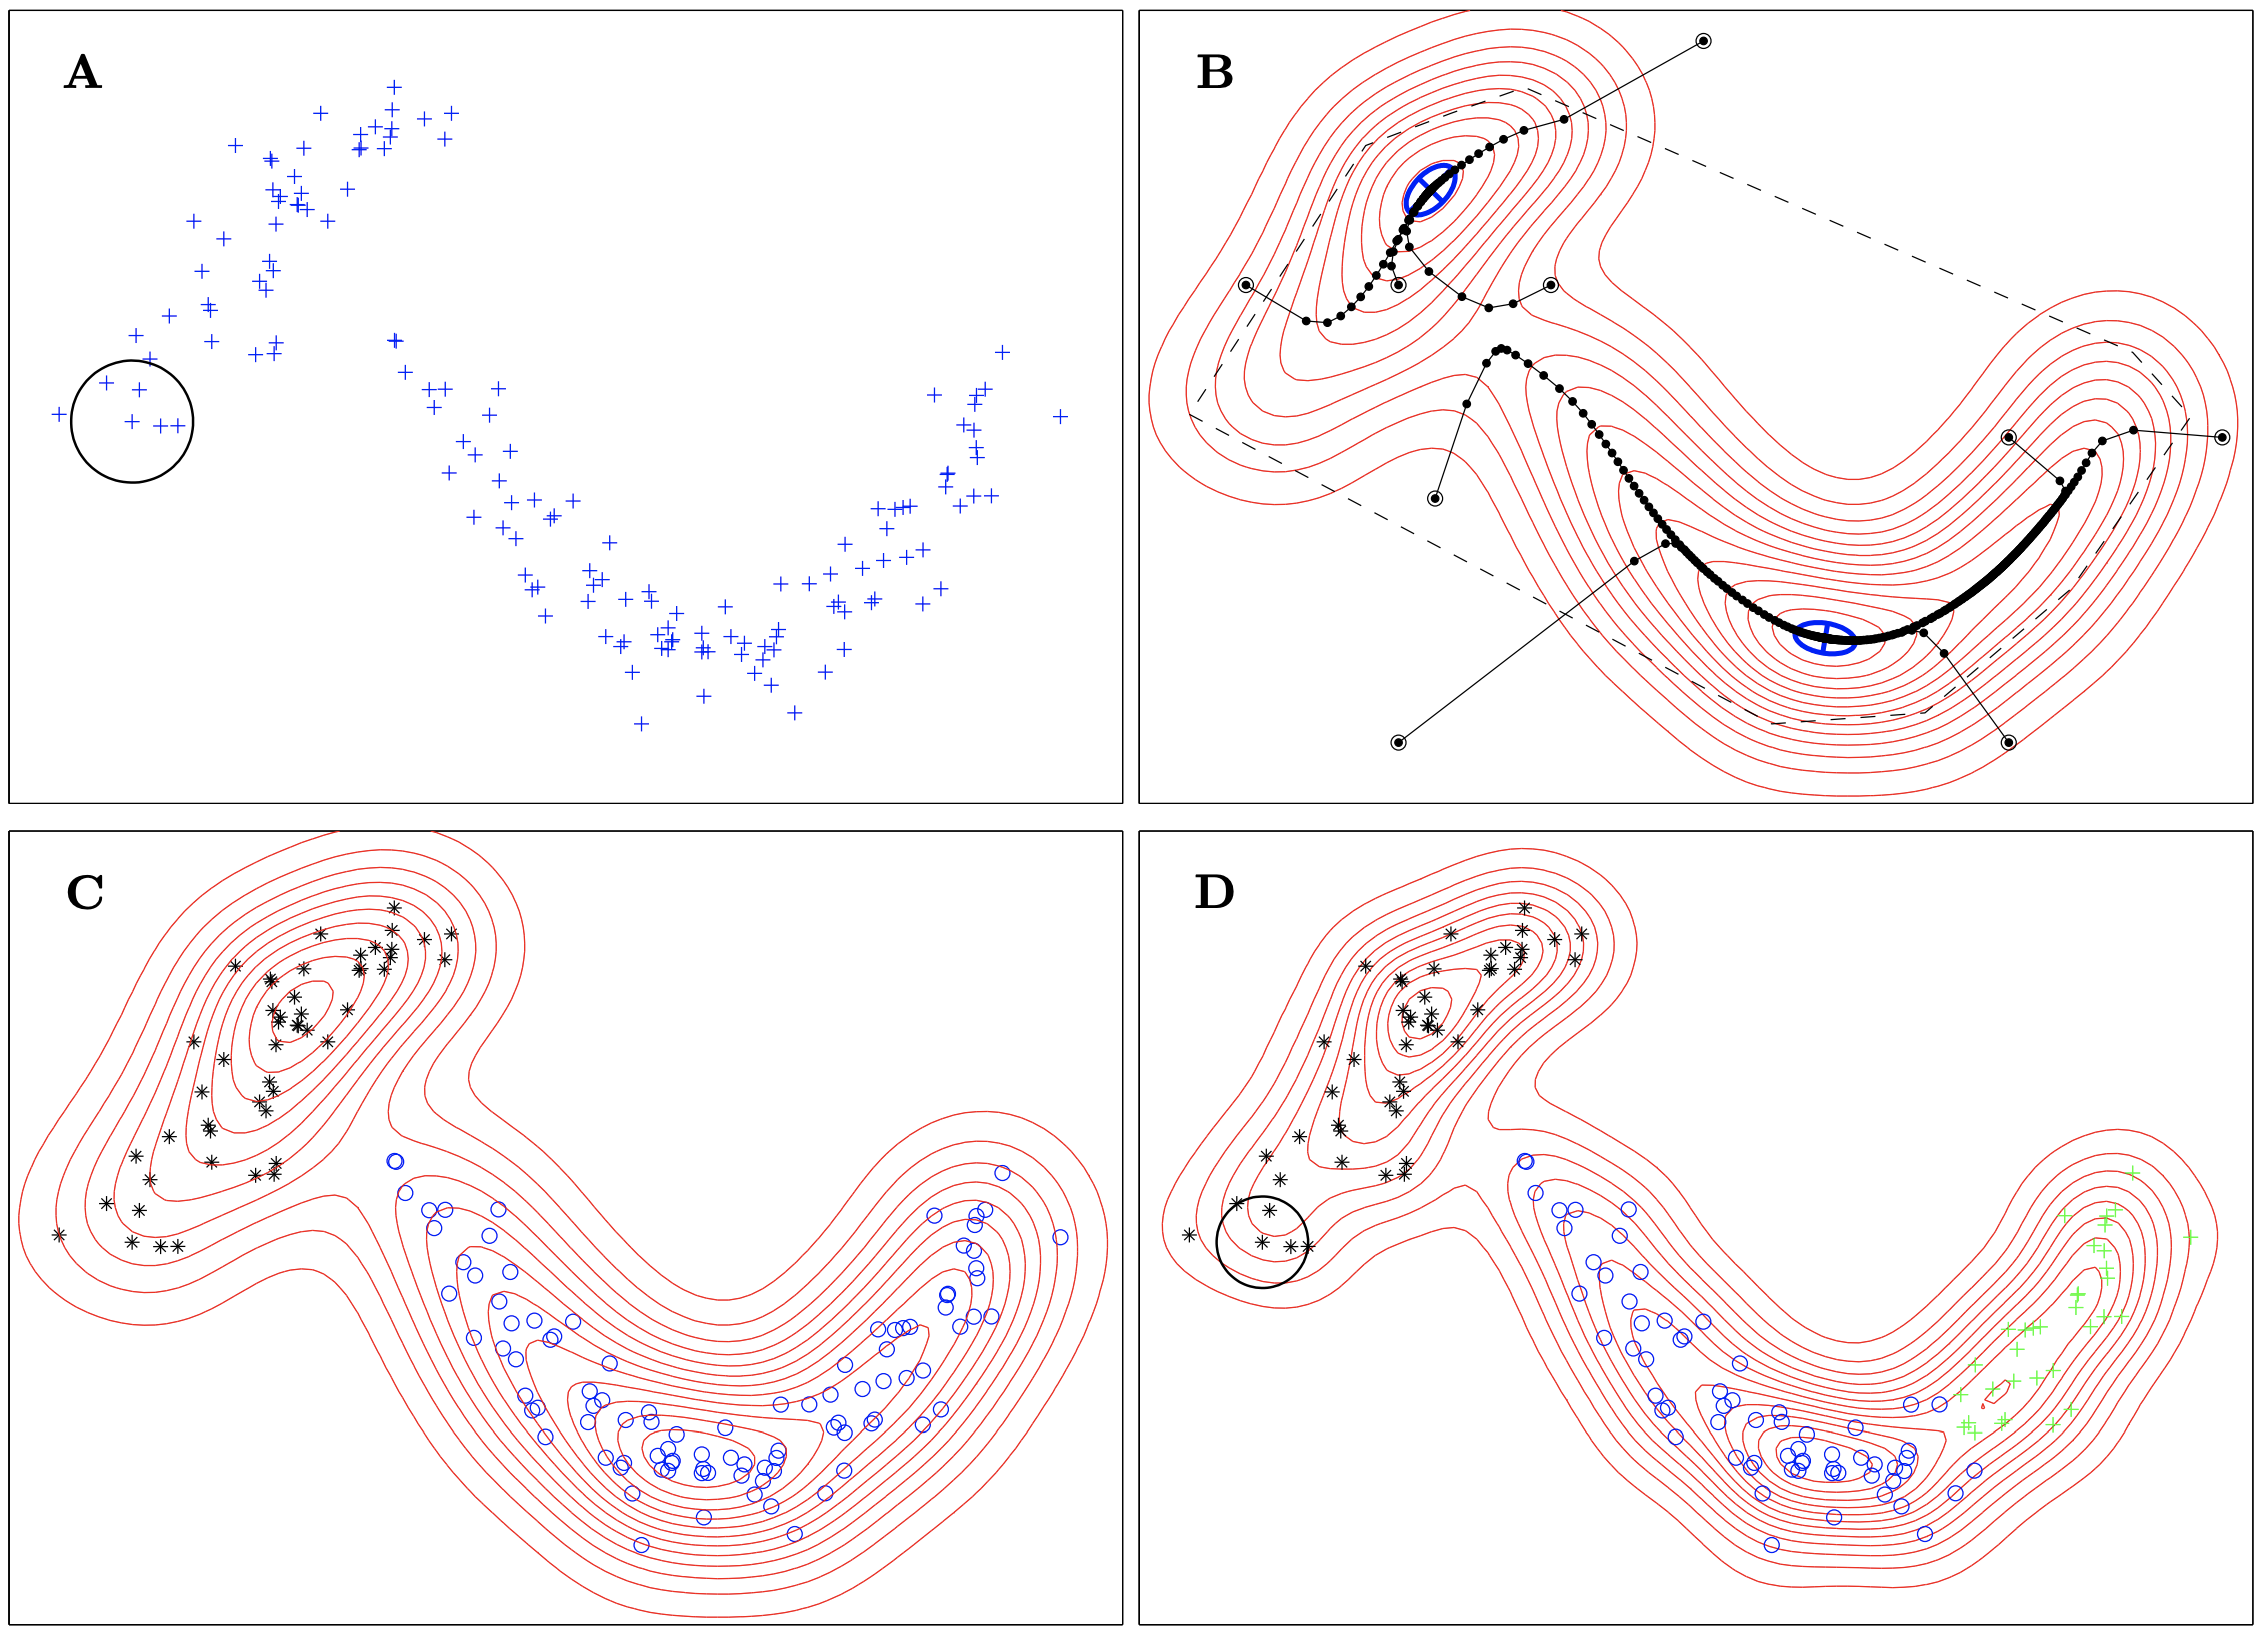
\includegraphics[width=\textwidth]{density_based_clustering.png}}
\caption{روند خوشه‌بندی یک الگوریتم تراکم‌محور\cite{carreira2015review}}
\label{fig:density_based_clustering}
\end{figure}

نحوه‌ی استفاده از این الگوریتم در این مسئله بدین گونه است که پیش از عملیات استخراج ویژگی‌ها و یادگیری ماشین، میانگین مقادیر لرزش در هر سه بعد برای هر اندازه‌گیری محاسبه می‌شود. این مقادیر نباید خیلی با هم اختلاف داشته باشند. برای تشخیص داده‌های پرت، خوشه‌بندی میانگین تغییر سه‌بعدی استفاده می‌کنیم و در نهایت داده‌هایی که در خوشه‌ی اقلیت قرار دارند را برای محاسبات و یادگیری ماشین در نظر نمی‌گیریم\cite{jung2017vibration}. برای پیاده‌سازی این الگوریتم کلاس \lr{MeanShiftClustering} در فایل \lr{clustering.py} پیاده‌شده است. این کلاس از کلاس \lr{MeanShift} از کتابخانه‌ی \lr{Scikit-Learn} ارث‌بری می‌کند.


\subsection{استخراج ویژگی‌ها}
تا اینجای کار، اثرهای انحرافات ممکن را از بین بردیم و داده‌های پرت را از میان کل داده‌ها جدا کردیم. از آنجا که داده‌ی خام لرزش گره‌های موجود در شبکه‌ی اشیاء، در دامنه‌ی زمانی\LTRfootnote{Time Domain} بوده و حالت شروع به کار و وضعیت فعلی هر کدام از آنها در حال حاضر با همدیگر متفاوت است، نیازمند آنیم که از این داده‌های خام، ویژگی‌هایی مناسب را جهت انجام تحلیل و یادگیری ماشین، استخراج کنیم؛ برای این منظور بردن داده‌های موجود در دامنه زمانی به دامنه‌ی فرکانسی با کمک تبدیل فوریه\LTRfootnote{Fourier Transform}، شروع خوبی است.

\subsubsection{ویژگی \lr{Root Mean Square (RMS)}}
ویژگی مربع میانگین ریشه یا به اختصار \lr{RMS} تنها بزرگی اندازه‌ی لرزش‌های اندازه‌ گرفته‌شده را نمایان می‌کند و برای بردارهای لرزش هر اندازه‌گیری منسوب به هر دستگاه اینترنت اشیاء موجود، به صورت \cref{eq:rms_feature} محاسبه می‌شود. در \cref{fig:rms} مقادیر محاسبه شده‌ی این ویژگی را برای همه‌ی اندازه‌گیری‌های یک گره موجود حساب کرده‌ایم. محور افقی شناسه‌ی هر یک از اندازه‌گیری‌ها می‌باشد.

\begin{equation}
\label{eq:rms_feature}
\begin{split} 
r^l_{nm} & = \dfrac{1}{\sqrt{K}}\|a^l_{nm}\|\\
r^2_{nm} &  = \sum_{l \in \{x, y, z\}} (r^l_{nm})^2
\end{split} 
\end{equation}


\begin{figure}[!h]
\centerline{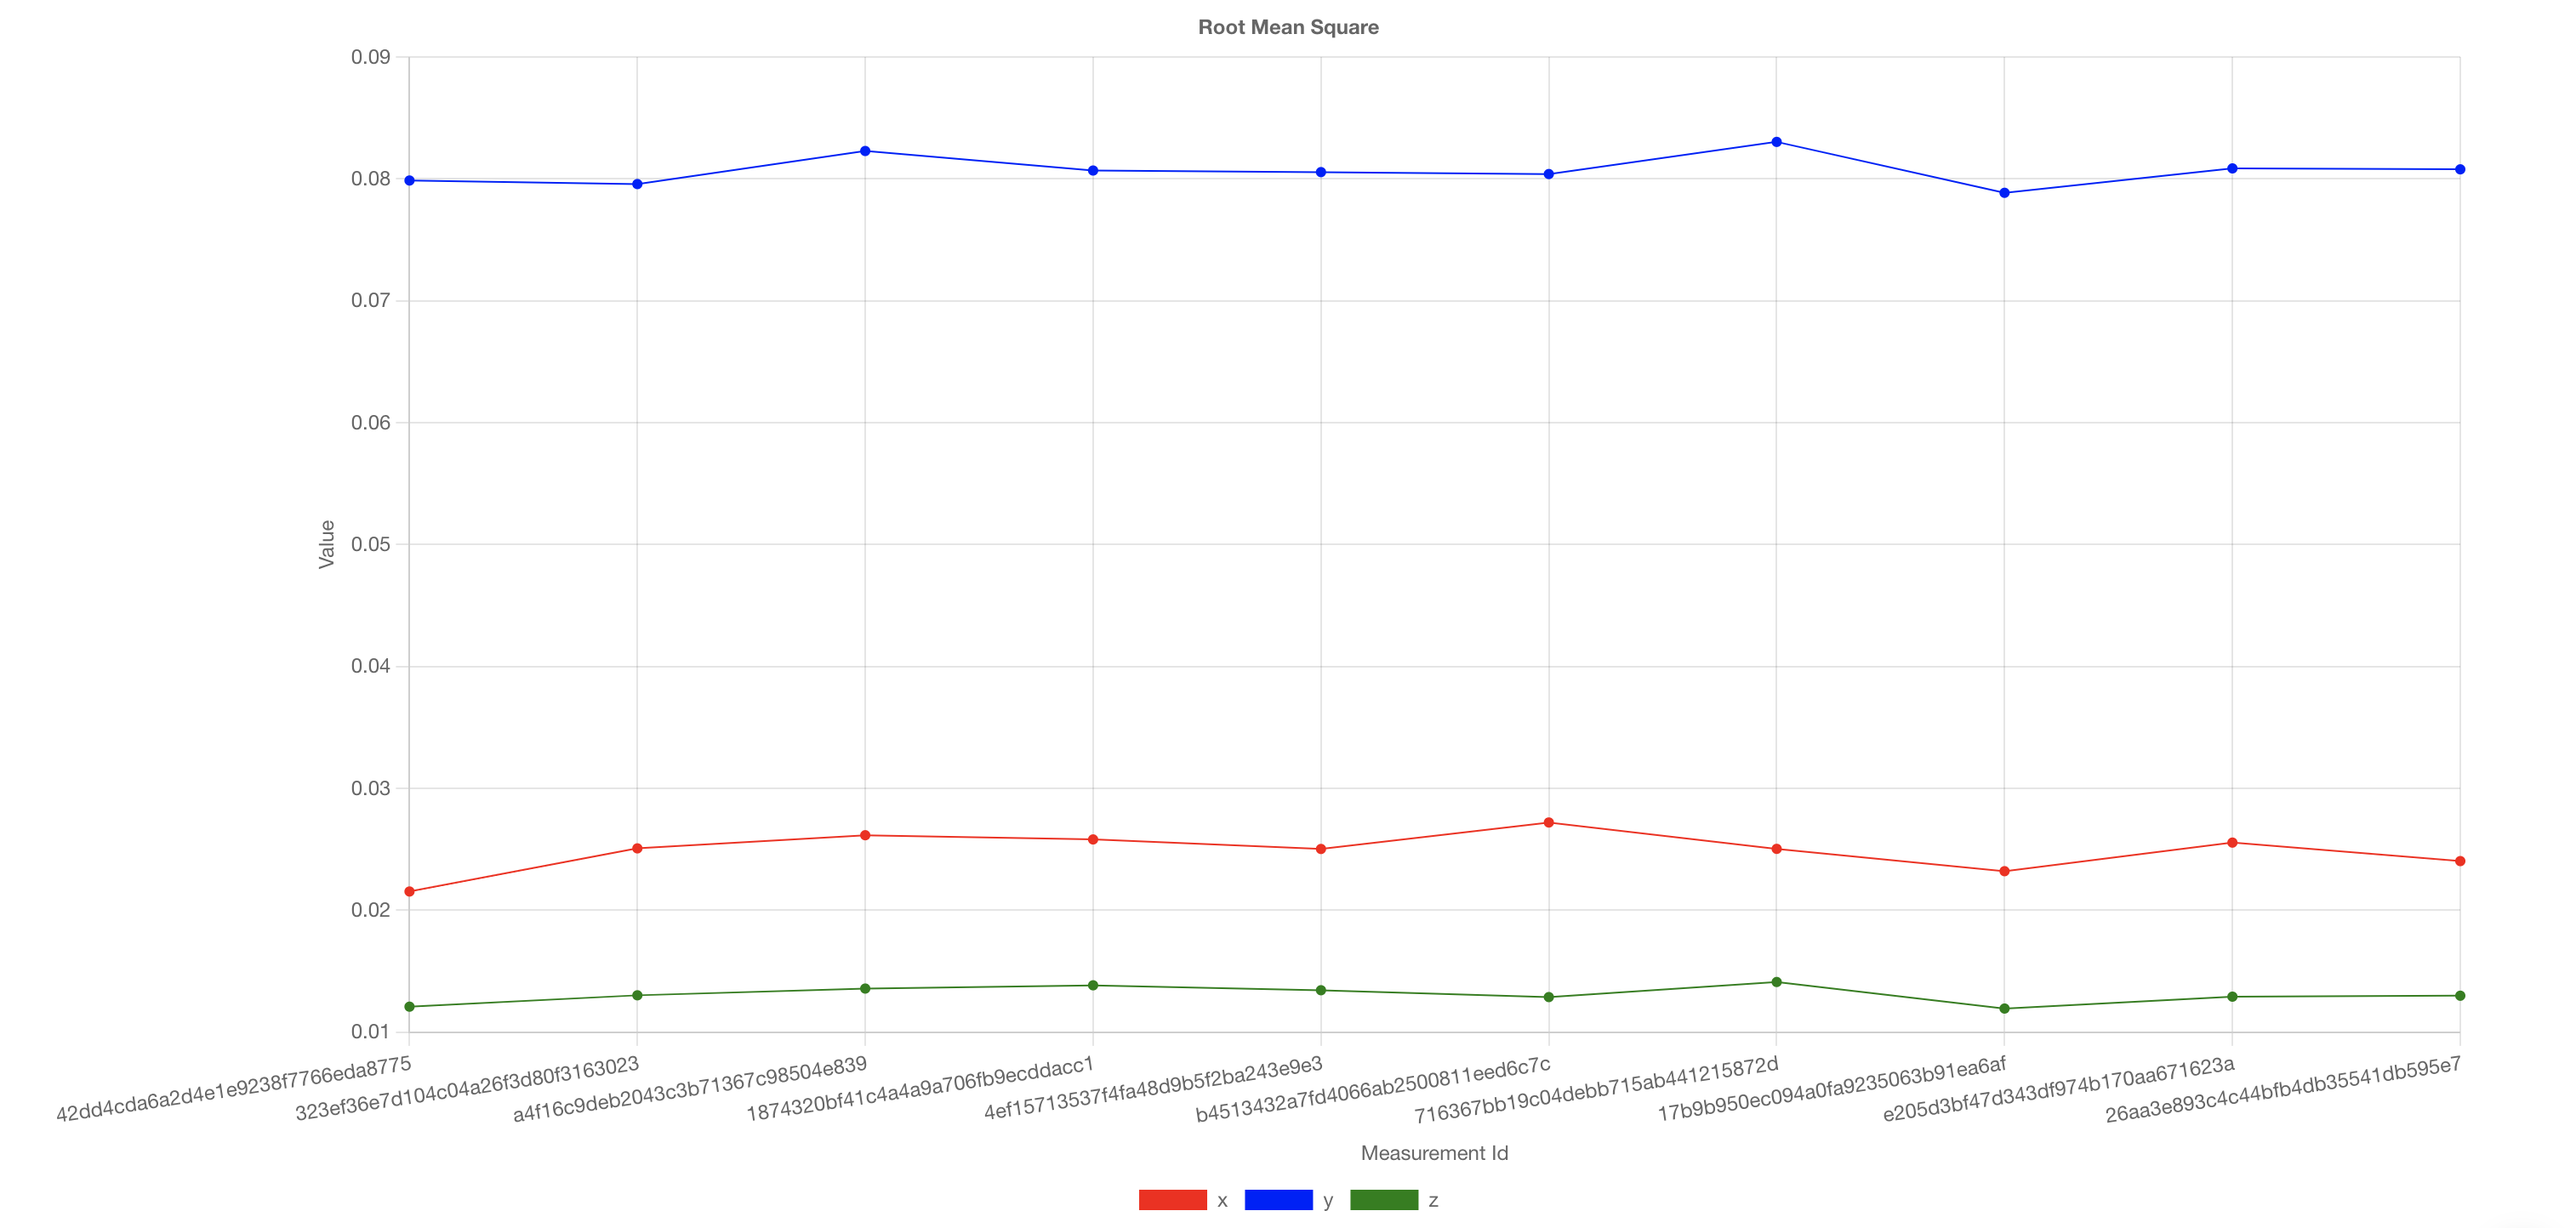
\includegraphics[width=\textwidth]{rms.png}}
\caption{مقادیر ویژگی مربع میانگین ریشه برای همه‌ی اندازه‌گیری‌های یک گره}
\label{fig:rms}
\end{figure}

همانطور که گفته‌شد این ویژگی اطلاعات زیادی را در اختیار ما قرار نمی‌دهد. نکته‌ی قابل توجه دیگر در مورد این ویژگی این است که مقادیر بدست آمده در این ویژگی منسوب به دامنه‌ی زمانی می‌باشد و با توجه به مسئله‌ی کنونی، این ویژگی کاربردی در تحلیل اطلاعات لرزش برای ما نخواهد داشت.


\subsubsection{ویژگی \lr{Power Spectral Density (PSD)}}
ویژگی چگالی طیفی توان یا \lr{PSD} به ما در یافتن مشخصه‌های مبهم موجود در ویژگی‌های مربوط به دامنه‌ی زمانی کمک می‌کند. با ضرب ماتریسی سیگنال لرزش اندازه‌گرفته شده در بعد زمان در یک ماتریس تبدیل کسینوسی گسسته\LTRfootnote{Discrete Cosine Transform (DCT)} به ابعاد $K \times K$، می‌توان بردار ویژگی سیگنال مربوطه را در حوزه‌ی فرکانس بدست آورد. در \cref{eq:psd_feature} طرز محاسبه‌ی این ویژگی را مشاهده می‌کنیم. نکته‌ی قابل توجه در این قسمت این است که بنابر قضیه‌ی پارسوال\LTRfootnote{Parseval's Theorem}، برابری $(r^l_{nm})^2 = \sum_{k = 1}^{K}s^l_{nmk}$ برقرار می‌باشد.

\begin{equation}
\label{eq:psd_feature}
\begin{split} 
s^l_{nm} & = \dfrac{1}{2K}(a^l_{nm} \times W_K)^2\\
s_{nm} &  = \sum_{l \in \{x, y, z\}} s^l_{nm}
\end{split} 
\end{equation}

 پس از این مرحله باید توجه کرد که ویژگی چگالی طیفی توان، یک ویژگی با ابعاد بالا (به اندازه‌ی تعداد نمونه‌ها در یک اندازه‌گیری که در مسئله‌ی ما این عدد برابر با ۶۰ می‌باشد) است که معمولا در هنگام محاسبات ($s^Ts$) منجر به ایجاد ماتریس منفرد\LTRfootnote{Singular Matrix} خواهد شد و در نتیجه برای مسائل رگرسیون دچار مشکل خواهیم شد. از طرف دیگر، این ویژگی به دلیل نوسانات تصادفی زیاد در دامنه آنها در فرکانس به دلیل انحراف اندازه گیری ذاتی در سنسور \lr{MEMS} غیرقابل اتکا است.
 
\subsubsection{ویژگی \lr{Harmonic Peaks Feature}}

برای رفع این مشکلات، ویژگی قله‌های موزون را معرفی می‌کنیم. برای هر اندازه‌گیری با ۶۰ نمونه، این ویژگی عبارت است از ۲۰ تا از بیشترین مقادیر ویژگی \lr{PSD} به همراه فرکانس‌های متناظر با آنها. به عبارت دیگر، این ویژگی به صورت $p_m = \{(f_{mk}, p_{mk})\}_{k=1, ..., n_p}$ تعریف می‌شود که $n_p$ در این مسئله برابر با ۲۰ است.

برای استخراج ویژگی قله‌های موزون، باید دو مرحله را طی کنیم.
\begin{itemize}
\item از بین بردن اثر انحرافات در اندازه‌گیری‌های ویژگی‌ \lr{PSD} با استفاده از عملیات پیچیدگی\LTRfootnote{Convolution} با پنجره‌ی هان\LTRfootnote{Hann Window} که در \cref{eq:hann_window} آورده شده است(در این برابری، $n_h$ اندازه‌ی پنچره است که در مسئله‌ی ما ۱۶ انتخاب شده است). پس از انجام این عملیات، سیگنال ویژگی‌ها هموار\LTRfootnote{Smooth} می‌شود و از این پس می‌توان عملیات جست‌وجو برای بیشترین مقادیر را شروع کرد.

\begin{equation}
\label{eq:hann_window}
w_h(n) = 0.5 (1 - \cos{\dfrac{2\pi n}{n_h - 1}})
\end{equation}

\item پیدا کردن ۲۰ تا از بیشترین مقادیر ویژگی‌های هموارشده از طریق شناسایی نقاطی که مشتق اول سیگنال در آنها از مثبت به منفی، تغییر علامت می‌دهد

\end{itemize}

در \cref{fig:psd} مقادیر ویژگی چگالی طیفی توان و ۲۰ تا از بیشترین قله‌های موزون را برای یکی از اندازه‌گیری‌های منسوب به یک گره، نمایش داده‌ایم.

\begin{figure}[!h]
\centerline{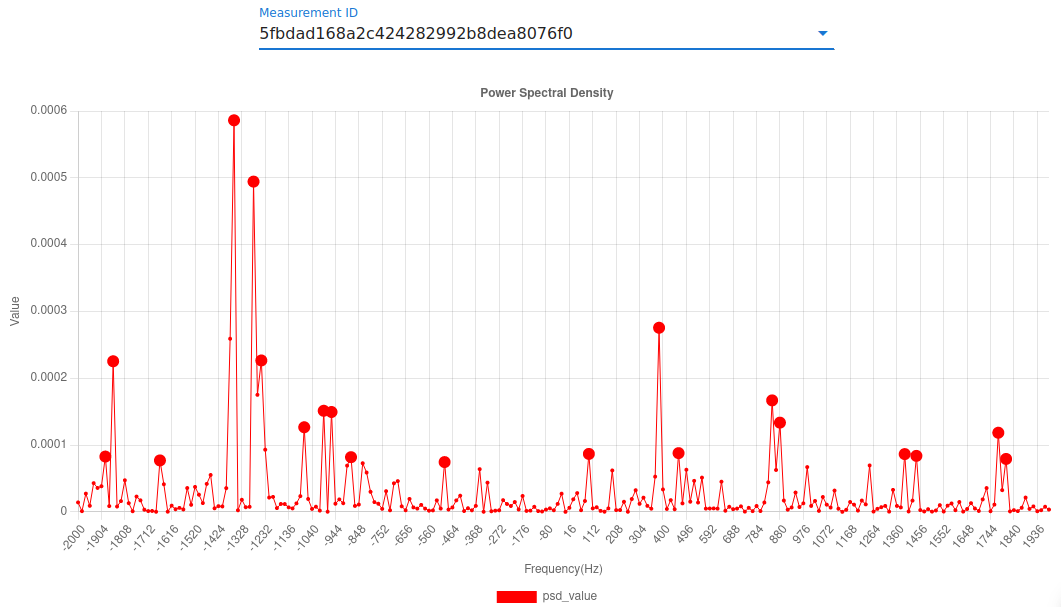
\includegraphics[width=\textwidth]{psd.png}}
\caption{مقادیر ویژگی چگالی طیفی توان و قله‌های موزون برای یک اندازه‌گیری از یک گره}
\label{fig:psd}
\end{figure}

\section{نحوه‌ی یادگیری مدل}
پس از استخراج ویژگی‌ها مناسب، نیازمند آنیم که با تحلیل این ویژگی‌ها به آموزش مدل بپردازیم. برای رسیدن به این مهم باید ابتدا روش مناسبی را برای مقایسه‌ی کمّی بین ویژگی‌های مختلف پیدا کرد. 

\subsection{محاسبه‌ی مشابهت بین وضعیت دستگاه‌ها}
در این مرحله، برای مشخص کردن میزان تفاوت بین دو ویژگی قله‌های موزون $p_i$ و $p_j$، \cref{alg:harmonic_peak_distance} را ارائه می‌دهیم. لازم به ذکر است که خروجی الگوریتم، $D_{ij}$، میزان عددی تفاوت بین ویژگی‌ها است و هرچه این عدد از صفر دورتر باشد، ویژگی‌ها متفاوت‌تر هستند\cite{jung2017vibration}.

\begin{algorithm}
\caption{تشخیص کمّی میزان تفاوت دو ویژگی}
\label{alg:harmonic_peak_distance}
\begin{latin}
\begin{algorithmic}
\Require $p_{max} \gets max(p_n, p_m), f_{max} \gets max(f_n, f_m)$  $\forall (p_n, f_n) \in p_i, \forall (p_m, f_m) \in p_j$
\Ensure $n_h = 16, n_p = 20$
\State $sum \gets 0, cnt \gets 0$
\State $p_n \gets p_n / p_{max},$  $f_n \gets f_n / f_{max},$  $\forall (p_n, f_n) \in p_i$
\State $p_m \gets p_m / p_{max},$  $f_m \gets f_m / f_{max},$  $\forall (p_m, f_m) \in p_j$
\State $queue_i \gets copy(p_i)$
\State $queue_j \gets copy(p_j)$
\While{$queue_i$ is not empty}
\State $(f_i, p_i) \gets queue_i.pop()$
\State {$f* \gets$ do binary search for $f_i$ in $[f_{j1} ... f_{j20}]$}
\If{$|f_i - f_{j*}| \times f_{max} < n_h$}
     \State $(f_{j*}, p_{j*}) \gets queue_j.pop(f_{j*})$
     \State $dist \gets dist + \|(f_i, p_i) - (f_{j*}, p_{j*})\|$
\Else
    \State $dist \gets \|(f_i, p_i)\|$
\EndIf
	\State $sum \gets sum + dist$
	\State $cnt \gets cnt + 1$
\EndWhile
\State $D_{ij} \gets (sum + \sum_{k=1}^{20} p_{jk}) / (cnt + len(p_j))$
\end{algorithmic}
\end{latin}
\end{algorithm}

\subsection{پیاده‌کردن مدل}
پس از طراحی \cref{alg:harmonic_peak_distance} تحلیل ویژگی‌های بدست آمده برای هر اندازه‌گیری را شروع می‌کنیم. نکته‌ی قابل توجه در این الگوریتم این است که این رویه، میزان جریمه‌ی بیشتری را برای مقادیر بیشینه در فرکانس‌های بالاتر در نظر می‌گیرد و این دقیقا همان چیزی است که به ما در شناسایی دستگاه‌های با کارکرد غیر عادی کمک می‌کند. از آنجا که این نوع دستگاه‌ها در فرکانس‌های بالاتر دچار انحرافات شدیدی هستند. در مقابل، دستگاه‌های با کارکرد عادی دارای مقادیر بیشینه‌ی بیشتر در فرکانس‌های پایین‌تر هستند.

با یک فرض پایه، توضیح نحوه‌ی یادگیری مدل را شروع می‌کنیم و آن این است که کلیه‌ی دستگاه‌ها به مرور زمان و با کار بیشتر، از حالت نویی دور می‌شوند. به عبارت دیگر، با گذشت زمان، هر دستگاه از وضعیت دستگاه تازه و آماده به کار دورتر می‌شود. برای این منظور، پارامتر $D_a$ را برای تحلیل دستگاه‌ها معرفی می‌کنیم که عبارت‌است از میزان متفاوت بودن دستگاه مورد نظر با یک 
دستگاه نو (کلاس کاری $A$ در \cref{table:node_state_labels}). تا زمانیکه هیچ نگهداری‌ای برای دستگاه صورت نگیرد، $D_a$ به مرور زمان به صورت یکنواخت افزایش می‌یابد.

\subsubsection{الگوریتم \lr{RANSAC}}

برای یادگیری این مدل خطی و پیش‌بینی زمان سرویس دستگاه‌ها از رویکرد اجماع نمونه‌ی تصادفی\LTRfootnote{RANdom SAmple Consensus (RANSAC)} یا به اختصار \lr{RANSAC} استفاده می‌کنیم. این الگوریتم، به صورت بازگشتی، مدل خطی‌ای بر اساس داده‌های آموزشی درست می‌کند و نکته‌ی قابل توجه این الگوریتم این است که توانایی تشخیص و در نظر نگرفتن داده‌های پرت را دارد و از این رو بسیار مناسب استفاده در این مسئله است. به طور کلی روند ایجاد مدل در این الگوریتم به صورت زیر است\cite{derpanis2010overview}:

\begin{enumerate}

\item به صورت تصادفی حداقل تعداد نقاط لازم، برای پیداکردن پارامترهای مدل مشخص می‌شود.
\item پارامتر‌های مدل بدست آورده می‌شوند.
\item از میان کل نقاط، تعداد نقاطی که با میزان تحمل از قبل تعیین شده‌ی $\epsilon$ شامل مدل هستند، حساب می‌شوند.
\item اگر نسبت نقاط مشمول در مدل به تعداد کل نقاط از یک مقدار از پیش‌ تعیین‌شده‌ی $\tau$ بیشتر شد، پارامتر‌های مدل دوباره با کمک نقاط مشمول حدس زده می‌شوند و الگوریتم پایان می‌یابد.
\item در غیر این صورت، مرحله‌ی ۱ تا ۴ تا حداکثر $N$ بار تکرار می‌شود.

\end{enumerate}

جهت پیش‌بینی میزان عمر مفید باقی‌مانده، الگوریتم ما ابتدا آستانه‌ی $D_a$ را برای دو کلاس کاری $B, C$ و $D$ حساب می‌کند. این آستانه از طریق کمینه کردن میزان خطا در طبقه‌بندی دستگاه‌های این دو کلاس مشخص می‌شود. پس از تعیین این آستانه، الگوریتم با بررسی مدل خطی بدست‌آمده از \lr{RANSAC}، میزان عمر مفید دستگاه مربوطه را خروجی‌ می‌دهد.

در \cref{fig:ransac_model}\cite{jung2017vibration} دو مدل برای پیش‌بینی میزان عمر مفید باقی‌مانده، آموزش داده‌شده است. محور افقی زمان اندازه‌گیری‌ها بر حسب روز و محور عمودی فاصله‌ی ویژگی‌های دستگاه‌ها با ویژگی دستگاه‌های سالم و نو است. همچنین خط بنفش‌رنگ، آستانه‌ی ورود دستگاه از کلاس دستگاه‌های سالم به کلاس دستگاه‌های معیوب می‌باشد (این مقدار آستانه در شکل برابر با ۰/۲۱ است). برای پیش‌بینی عمر باقی‌مانده‌ی هر دستگاه ابتدا میزان تعلق مقادیر $D_a$ برای آن دستگاه در دو مدل محاسبه می‌شود. سپس این حد آستانه با مدلی که دستگاه بیشترین تعلق را به آن دارد تلاقی داده می‌شود. در نهایت فاصله‌ی زمان اندازه‌گیری با نقطه‌ی تلاقی، برابر با عمر مفید باقی‌مانده‌ی دستگاه مورد نظر بر حسب روز است.

\begin{figure}[!h]
\centerline{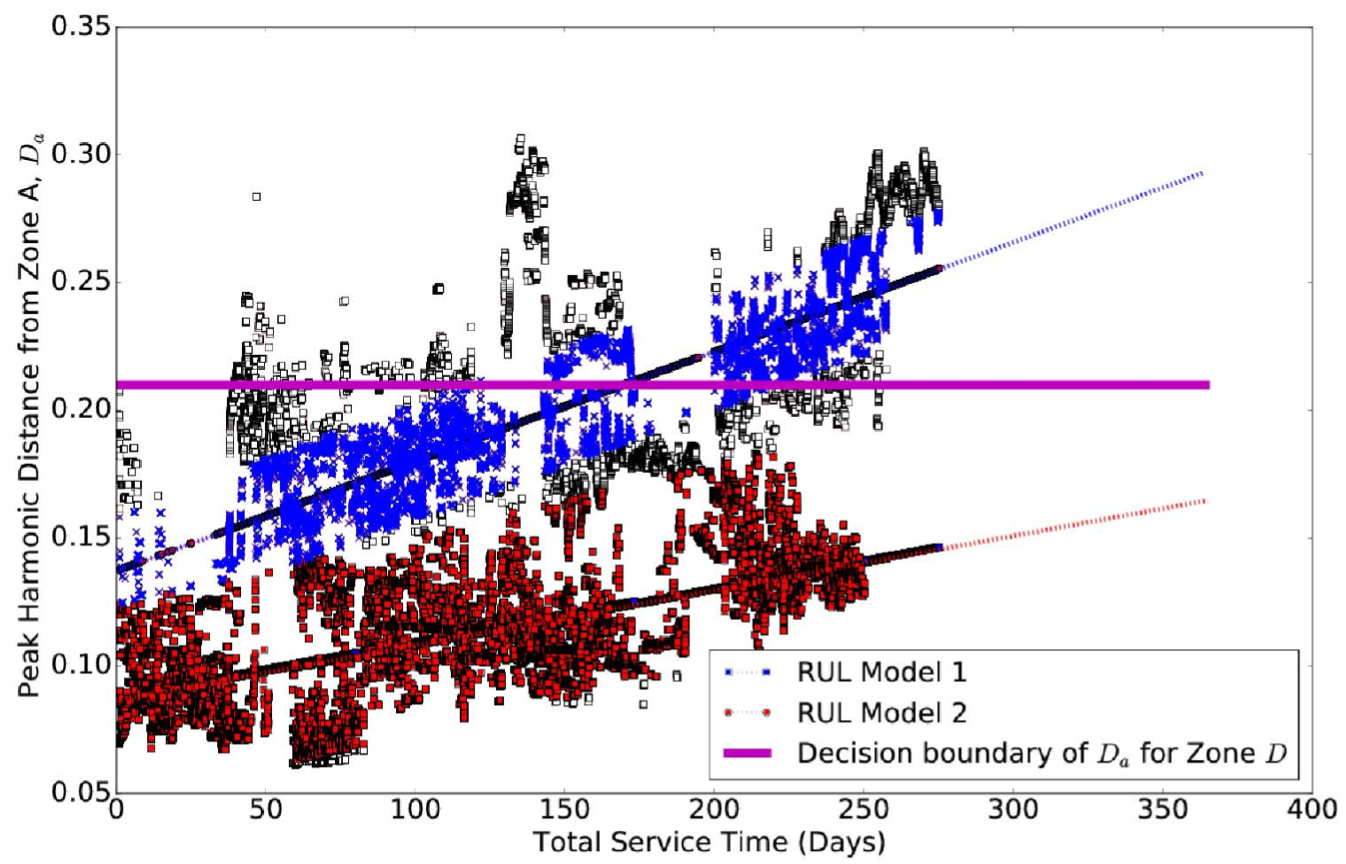
\includegraphics[width=0.7\textwidth]{ransac_model.png}}
\caption{دو مدل یادگیری ماشین برای مسئله‌ی پیش‌بینی میزان عمر مفید باقی‌مانده\cite{jung2017vibration}}
\label{fig:ransac_model}
\end{figure}

\section{جمع‌بندی و نتیجه‌گیری}
این بخش به طور دقیق روند یادگیری ماشین از اطلاعات لرزش گره‌ها را نشان داد. مشخص شد که داده‌های جمع‌آوری شده ابتدا به کمک پیش‌پردازنده که شامل هنجارکننده، تشخیص‌دهنده‌ی داده‌ی پرت و استخراج‌کننده‌ی ویژگی‌های آماده پردازش است، پالایش شده و سپس تحویل واحد یادگیری ماشین می‌شود. در این مرحله این واحد ابتدا با هموار کردن و سپس با انتخاب کردن ۲۰ تا از بیشترین مقادیر موزون ویژگی \lr{PSD} برای هر اندازه‌گیری، اقدام به محاسبه‌ی میزان شباهت این اندازه‌گیری‌ها به اندازه‌گیری‌های یک دستگاه سالم می‌کند و بنا به میزان شباهت یا تفاوت با آن، پیش‌بینی مربوط به طول عمر باقی‌مانده‌ی گره را خروجی خواهد داد.

%--------------------------------------------------------------------------appendix( مراجع و پیوست ها)
\chapterfont{\vspace*{-2em}\centering\LARGE}%

\appendix
\bibliographystyle{plain-fa}
\bibliography{references}
\chapter*{‌پیوست}
\markboth{پیوست}{}
\addcontentsline{toc}{chapter}{پیوست}
موضوعات مرتبط با متن گزارش پایان نامه كه در يكی از گروه‌های زير قرار می‌گيرد، در بخش پيوست‌ها آورده شوند:
\begin{enumerate}
\item  اثبات های رياضی يا عمليات رياضی طولانی‌.‌
\item داده و اطلاعات نمونه (های) مورد مطالعه (\lr{Case Study}) چنانچه طولانی باشد‌.‌
\item نتايج كارهای ديگران چنانچه نياز به تفصيل باشد‌.‌
\item مجموعه تعاريف متغيرها و پارامترها، چنانچه طولانی بوده و در متن به انجام نرسيده باشد‌.‌
\end{enumerate}
% براي شماره‌گذاري روابط، جداول و اشكال موجود در پيوست‌ از ساختار متفاوتي نسبت به متن اصلي استفاده مي‌شود كه در زير به‌عنوان نمونه نمايش داده شده‌است. 
% \begin{equation}
%F=ma
%\end{equation}
\section*{کد میپل }
\begin{latin}
\begin{verbatim}

with(DifferentialGeometry):
with(Tensor):
DGsetup([x, y, z], M)
																	frame name: M
a := evalDG(D_x)
																	D_x
b := evalDG(-2 y z D_x+2 x D_y/z^3-D_z/z^2)


\end{verbatim}
\end{latin}
%--------------------------------------------------------------------------dictionary(واژه نامه ها)
%اگر مایل به داشتن صفحه واژه‌نامه نیستید، خط زیر را غیر فعال کنید.
\parindent=0pt
%
\chapter*{واژه‌نامه‌ی فارسی به انگلیسی}
\pagestyle{style9}

\addcontentsline{toc}{chapter}{واژه‌نامه‌ی فارسی به انگلیسی}
%%%%%%
\begin{multicols*}{2}

{\bf آ}
\vspace*{3mm}


\farsiTOenglish{اسکالر}{Scalar}


\vspace*{3mm}
{\bf ب}
\vspace*{3mm}

\farsiTOenglish{بالابر}{Lift}


\vspace*{3mm}
{\bf پ}
%%\vspace*{3mm}

\farsiTOenglish{پایا}{Invariant}



\vspace*{3mm}
{\bf ت}
%%\vspace*{3mm}

\farsiTOenglish{ تناظر }{Correspondence}


\vspace*{3mm}
{\bf ث}
%%\vspace*{3mm}

\farsiTOenglish{ثابت‌ساز}{Stabilizer}

\vspace*{3mm}
{\bf ج}
%%\vspace*{3mm}

\farsiTOenglish{جایگشت}{Permutation}



\vspace*{3mm}
{\bf چ}
%%\vspace*{3mm}


\farsiTOenglish{چند جمله‌ای }{Polynomial}

\vspace*{3mm}
{\bf ح}
%%\vspace*{3mm}

\farsiTOenglish{حاصل‌ضرب دکارتی}{Cartesian product}


\vspace*{3mm}
{\bf خ}
%%\vspace*{3mm}

\farsiTOenglish{خودریختی}{Automorphism}

\vspace*{3mm}
{\bf د}
%%\vspace*{3mm}

\farsiTOenglish{درجه}{Degree}


\vspace*{3mm}
{\bf ر}
%%\vspace*{3mm}


\farsiTOenglish{ریزپردازنده}{microprocessor}


\vspace*{3mm}
{\bf ز}
%%\vspace*{3mm}


\farsiTOenglish{زیرمدول}{Submodule}


\vspace*{3mm}
{\bf س}
%%\vspace*{3mm}

\farsiTOenglish{سرشت}{Character}


\vspace*{3mm}
{\bf ص}
%%\vspace*{3mm}

\farsiTOenglish{صادقانه}{Faithful}

\vspace*{3mm}
{\bf ض}
%%\vspace*{3mm}

\farsiTOenglish{ضرب داخلی}{Inner product}

\vspace*{3mm}
{\bf ط}
%%\vspace*{3mm}


\farsiTOenglish{طوقه}{Loop}


\vspace*{3mm}
{\bf ظ}
%%\vspace*{3mm}


\farsiTOenglish{ظرفیت}{Valency}
 
\vspace*{3mm}
{\bf ع}
%%\vspace*{3mm}


\farsiTOenglish{عدم مجاورت}{Nonadjacency}



\vspace*{3mm}
{\bf ف}
%%\vspace*{3mm}

\farsiTOenglish{فضای برداری}{Vector space}



\vspace*{3mm}
{\bf ک}
%%\vspace*{3mm}

\farsiTOenglish{کاملاً تحویل‌پذیر}{Complete reducibility}


\vspace*{3mm}
{\bf گ}
%%\vspace*{3mm}


\farsiTOenglish{گراف}{Graph}



\vspace*{3mm}
{\bf م}
%%\vspace*{3mm}

\farsiTOenglish{ماتریس جایگشتی}{Permutation matrix }


\vspace*{3mm}
{\bf ن}
%%\vspace*{3mm}

\farsiTOenglish{ناهمبند}{Disconnected}


\vspace*{3mm}
{\bf و}
%%\vspace*{3mm}

\farsiTOenglish{وارون‌پذیر}{Invertible}


\vspace*{3mm}
{\bf ه}
%%\vspace*{3mm}

\farsiTOenglish{همبند}{Connected}



\vspace*{3mm}
{\bf ی}
%%\vspace*{3mm}

\farsiTOenglish{یال}{Edge}




\end{multicols*}%
%%%%%%
\chapter*{ واژه‌نامه‌ی انگلیسی به فارسی}
\pagestyle{style9}
\lhead{\thepage}\rhead{واژه‌نامه‌ی انگلیسی به فارسی}
\addcontentsline{toc}{chapter}{واژه‌نامه‌ی انگلیسی به فارسی}

\LTRmulticolcolumns
\begin{multicols}{2}
{\hfill\bf  \lr{A}}
%%\vspace*{1.5mm}

\englishTOfarsi{Automorphism}{خودریختی}

\vspace*{3mm}
{\hfill\bf   \lr{B}}
%%\vspace*{1.5mm}

\englishTOfarsi{Bijection}{دوسویی}

\vspace*{3mm}
{\hfill\bf   \lr{C}}
%%\vspace*{1.5mm}

\englishTOfarsi{Cycle group}{گروه دوری}

\vspace*{3mm}
{\hfill\bf   \lr{D}}
%%\vspace*{1.5mm}

\englishTOfarsi{Degree}{درجه}

\vspace*{3mm}
{\hfill\bf   \lr{E}}
%%\vspace*{1.5mm}

\englishTOfarsi{Edge}{یال}

\vspace*{3mm}
{\hfill\bf   \lr{F}}
%%\vspace*{1.5mm}

\englishTOfarsi{Function}{تابع}

\vspace*{3mm}
{\hfill\bf   \lr{G}}
%%\vspace*{1.5mm}

\englishTOfarsi{Group}{گروه}

\vspace*{3mm}
{\hfill\bf   \lr{H}}
%%\vspace*{1.5mm}

\englishTOfarsi{Homomorphism}{همریختی}

\vspace*{3mm}
{\hfill\bf   \lr{I}}
%%\vspace*{1.5mm}

\englishTOfarsi{Invariant}{پایا}

\vspace*{3mm}
{\hfill\bf   \lr{L}}
%%\vspace*{1.5mm}

\englishTOfarsi{Lift}{بالابر}

\vspace*{3mm}
{\hfill\bf   \lr{M}}
%%\vspace*{1.5mm}

\englishTOfarsi{Module}{مدول}

\vspace*{3mm}
{\hfill\bf   \lr{N}}
%%\vspace*{1.5mm}

\englishTOfarsi{Natural map}{نگاشت طبیعی}

\vspace*{3mm}
{\hfill\bf   \lr{O}}
%%\vspace*{1.5mm}

\englishTOfarsi{One to One}{یک به یک}

\vspace*{3mm}
{\hfill\bf   \lr{P}}
%%\vspace*{1.5mm}

\englishTOfarsi{Permutation group}{گروه جایگشتی}

\vspace*{3mm}
{\hfill\bf   \lr{Q}}
%%\vspace*{1.5mm}

\englishTOfarsi{Quotient graph}{گراف خارج‌قسمتی}

 \vspace*{3mm}
{\hfill\bf   \lr{R}}
%%\vspace*{1.5mm}

\englishTOfarsi{Reducible}{تحویل پذیر}

\vspace*{3mm}
{\hfill\bf   \lr{S}}
%%\vspace*{1.5mm}

\englishTOfarsi{Sequence}{دنباله}

 \vspace*{3mm}
{\hfill\bf   \lr{T}}
%%\vspace*{1.5mm}

\englishTOfarsi{Trivial character}{سرشت بدیهی}

\vspace*{3mm}
{\hfill\bf   \lr{U}}
%%\vspace*{1.5mm}

\englishTOfarsi{Unique}{منحصربفرد}

\vspace*{3mm}
{\hfill\bf   \lr{V}}
%%\vspace*{1.5mm}

\englishTOfarsi{Vector space}{فضای برداری}
\end{multicols}
%--------------------------------------------------------------------------index(نمایه)
%اگر مایل به داشتن صفحه نمایه نیستید، خط زیر را غیر فعال کنید.
\pagestyle{style7}
\printindex
\pagestyle{style7}
%کلمات کلیدی انگلیسی
\latinkeywords{Write a 3 to 5 KeyWords is essential. Example: AUT, M.Sc., Ph. D,..}
%چکیده انگلیسی

\en-abstract{
This page is accurate translation from Persian abstract into English.
}
%%%%%%%%%%%%%%%%%%%%% کدهای زیر را تغییر ندهید.

\newpage
\thispagestyle{empty}
\begin{latin}
\section*{\LARGE\centering Abstract}

\een-abstract

\vspace*{.5cm}
{\large\textbf{Key Words:}}\par
\vspace*{.5cm}
\elatinkeywords
\end{latin}
% در این فایل، عنوان پایان‌نامه، مشخصات خود و چکیده پایان‌نامه را به انگلیسی، وارد کنید.
%%%%%%%%%%%%%%%%%%%%%%%%%%%%%%%%%%%%
\baselineskip=.6cm
\begin{latin}

\latinfaculty{Department of Computer Engineering}


\latintitle{A Vibration Sensor Data Gathering System for IoT-based Predictive Maintenance}


\firstlatinsupervisor{Dr. Hamidreza Zarandi}

%\secondlatinsupervisor{Second Supervisor}

\firstlatinadvisor{Dr. Hamed Farbeh}

%\secondlatinadvisor{Second Advisor}

\latinname{Arian}

\latinsurname{Boukani}

\latinthesisdate{May 2023}

\latinvtitle
\end{latin}

\end{document}